\documentclass[aspectratio=169]{beamer}
\usepackage[utf8]{inputenc}
\usepackage[T1]{fontenc}
\usepackage{hyperref}
\usepackage{booktabs}
\usepackage{graphicx}
\usepackage{caption}
\usepackage{subcaption}
\usepackage{float}
\usepackage{multirow}
\usepackage{subcaption}
\usepackage{algorithm}
\usepackage[noend]{algpseudocode}
\usepackage{amssymb}
\usepackage{amsmath}
\usepackage{pifont}
\usepackage{cleveref}
\usepackage{mathabx}
\usepackage{mathpazo}
\usepackage{eulervm}
\usepackage{natbib}
\usepackage{listings}
\usepackage{color}
\usepackage[export]{adjustbox}
\usepackage{appendixnumberbeamer}
\usetheme{pro}
\newcommand{\cmark}{\ding{51}}
\newcommand{\xmark}{\ding{55}}
\newcommand{\eop}{\vspace{10px}}
\renewcommand{\sf}[1]{\textsf{\textup{#1}}}  
\renewcommand{\tt}[1]{\texttt{\textup{#1}}}  
\definecolor{mygreen}{rgb}{0,0.6,0}
\definecolor{mygray}{rgb}{0.5,0.5,0.5}
\definecolor{mymauve}{rgb}{0.58,0,0.82}
\newcommand{\g}[1]{{\color{green}#1}}
\renewcommand{\b}[1]{{\color{blue}#1}}
\renewcommand{\r}[1]{{\color{red}#1}}  

\lstset{ 
  % backgroundcolor=\color{white},   % choose the background color; you must add \usepackage{color} or \usepackage{xcolor}; should come as last argument
  basicstyle=\footnotesize,        % the size of the fonts that are used for the code
  breakatwhitespace=false,         % sets if automatic breaks should only happen at whitespace
  breaklines=true,                 % sets automatic line breaking
  captionpos=b,                    % sets the caption-position to bottom
  commentstyle=\color{mygreen},    % comment style
  deletekeywords={...},            % if you want to delete keywords from the given language
  escapeinside={\%*}{*)},          % if you want to add LaTeX within your code
  extendedchars=true,              % lets you use non-ASCII characters; for 8-bits encodings only, does not work with UTF-8
  firstnumber=1,                   % start line enumeration with line 1000
  frame=single,	                   % adds a frame around the code
  keepspaces=true,                 % keeps spaces in text, useful for keeping indentation of code (possibly needs columns=flexible)
  keywordstyle=\color{blue},       % keyword style
  language=Octave,                 % the language of the code
  morekeywords={*,...},            % if you want to add more keywords to the set
  numbers=left,                    % where to put the line-numbers; possible values are (none, left, right)
  numbersep=5pt,                   % how far the line-numbers are from the code
  numberstyle=\tiny\color{mygray}, % the style that is used for the line-numbers
  rulecolor=\color{black},         % if not set, the frame-color may be changed on line-breaks within not-black text (e.g. comments (green here))
  showspaces=false,                % show spaces everywhere adding particular underscores; it overrides 'showstringspaces'
  showstringspaces=false,          % underline spaces within strings only
  showtabs=false,                  % show tabs within strings adding particular underscores
  stepnumber=1,                    % the step between two line-numbers. If it's 1, each line will be numbered
  stringstyle=\color{mymauve},     % string literal style
  % tabsize=2,	                   % sets default tabsize to 2 spaces
  % title=\lstname                 % show the filename of files included with \lstinputlisting; also try caption instead of title
}
%% Load the markdown package
\usepackage[citations,footnotes,definitionLists,hashEnumerators,smartEllipses,tightLists=false,pipeTables,tableCaptions,hybrid,fencedCode]{markdown}
%%begin novalidate
\markdownSetup{rendererPrototypes={
    link = {\href{#2}{#1}},
    headingOne = {\section{#1}},
    headingTwo = {\subsection{#1}},
    headingThree = {\begin{frame}\frametitle{#1}},
    headingFour = {\begin{block}{#1}},
    horizontalRule = {\end{block}}
}}
%%end novalidate
\begin{document}
\title[BigData (Module 2)]{Cloud architectures for big data}
\date[DOLAP]{2021}
\author[Matteo Francia (UniBO)]{
    \textit{\textbf{Matteo Francia}}\inst{1}\\
    \url{m.francia@unibo.it}
}
\institute[UniBO]{\inst{1} University of Bologna}

\begin{frame}
\titlepage
\end{frame}

% \AtBeginSubsection[]{
%     \frame<beamer>{
%     \frametitle{Outline}   
%     \tableofcontents[
%         currentsection,
%         currentsubsection,
%         sectionstyle=show/hide,
%         subsectionstyle=show/shaded/hide,
%         subsubsectionstyle=show/show/shaded/shaded
%     ]}
% }

\begin{frame}{Organization}
10 hours
\begin{itemize}
    \item  4h (theory) on cloud computing and architectures + introduction to case study
    \item  3h (lab) case study on-premises
    \item  3h (lab) case study Amazon AWS
    \item  3h seminario (case study vero, pricing, etc.) ???
\end{itemize}
\end{frame}

\frame{\tableofcontents}
\setlength{\parskip}{1em}

\begin{frame}[allowframebreaks]{So far...}
You've practiced with on-premises solutions

Open questions?
\i How do we set up independent services?
\i How do we integrate such services?
\i How do we interface the services?

Let's guess
\i How would you do that?
\i How much time would it take?

\framebreak

No easy answers

Big-data (distributed) architectures require \textit{a lot} of skills
\i installation: how do i cable dozens cluster?
\i management: how do i replace a broken disk?
\i installation: how do i set up a new machine?
\i upgrade: how do i extend the cluster with new services/machines?
\i (energy and cooling, networking, software licenses, insurance...)

\framebreak

Technological perspective
\i it depends on your (team) skills (not only software engineering)
\si how do we orchestrate data flows?
\si how do control resource accesses (e.g., storage)?
\si how do we configure a distributed environment?

Business perspective
\i no free lunch, each choice as cost/benefit
\si how much time does it take to master a technology?
\si how many people do i need?

\framebreak

Can we afford to spend resources on tasks are not core for our mission?
\i mission: a statement used by a company to explain its purpose(s)

How can I build a working application/data platform?

\end{frame}

\sec{Cloud computing and big data}

\ssec{Why going cloud}

\begin{frame}

\includegraphics[width=\textwidth]{imgs/xkcd_cloud.png}
\end{frame}

\begin{frame}{Definition}
\begin{block}{Cloud computing (National Institute of Standards and Technology, NIST)}
A model for enabling ubiquitous, convenient, on-demand network access to a shared pool of configurable computing resources (e.g., networks, servers, storage, services) that can be rapidly provisioned and released with minimal management effort or service provider interaction. 
\end{block}

\i On-demand self-service (consume services when you want)
\i Broad network access (consume services from anywhere)
\i Resource pooling (infrastructure, virtual platforms, and applications)
\i Having big pools of resources enables economy of scale
\i Rapid elasticity (enable horizontal scalability)
\i Measured service (pay for the service you consume as you consume)
\end{frame}

\begin{frame}[allowframebreaks]{Why going cloud?}
\textbf{Scalability} that is not possible on premises
\si scale from one server to thousands
of servers
\si grow storage from gigabytes to petabytes
\si no longer think about rack space, switches, and power supplies

\textbf{Reliability} 
\i built to handle failures
\i fault-tolerant or highly available

\framebreak

\textbf{Resource pooling}
\i enable a resource to serve different consumers
\i dynamically assigned and reassigned according to demands
\i economy of scale

\textbf{Elasticity}
\i automated ability to scale resources in response to run-time conditions
\i core justification for the adoption of cloud

\framebreak

Worldwide \textbf{deployment}
\i deploy applications as close to customers as possible
\i improve data locality and privacy

Service \textbf{integration}
\i services solve common problems (e.g., load balancing, queuing)
\i do not reinvent the wheel

User perspective
\i eliminate repetitive tasks to focus on strategic ones
\i adapt infrastructure to requirements, create (test) environments on demand
\i abstract the underlying architecture

\framebreak

Service \textbf{integration} and \textbf{abstraction} are drivers of change
\i From databases to data plaforms
\i From on-premises hardware to serverless architectures

\end{frame}

\sssec{Data platform}
\begin{frame}[allowframebreaks]{Data platform}

Companies are collecting huge volumes of data to enable advanced analytics 
\i Data are more and more heterogeneous and complex
\i Databases/warehouses are no  longer ideal data hubs for integration/analysis

However, 
\i Raw data are difficult to obtain, interpret, describe, and maintain
\i There is a need for describing/curating the data to make them consumable

Data lakes (DLs) have increasingly taken the role of such hubs
\i Eliminate up-front costs of ingestion since data are stored in original format
\i Once in DL, data are available for analysis by everyone in the organization

\framebreak

However, 
\i getting  value  from  data  is  not  only  a  matter of storage
\i need integrated and multilevel analytical skills and techniques

Couto et al.: \textit{"A DL is a \b{central} repository system for \r{storage, processing, and analysis} of raw data, in which the data is kept in its original format and is \g{processed to be queried only when needed}.  It can store a varied amount of formats in big data ecosystems, from unstructured, semi-structured, to structured data sources."}

\framebreak

Drawing a sharp line been storage/computation/analysis is hard
\i Is a database just storage?
\i What about SQL?
\i What about OLAP?

Blurring of the architectural borderlines
\i ``DL'' is often replaced by ``data platform'' or ``data ecosystem''
\i encompass systems supporting data-intensive storage, computation, analysis

(Cloud-based) Data platform (e.g., Google and Amazon)
\i rationale: relieve users from complexity of administration and provision
\si not only technological skills, but also privacy, access control, etc.
\si only focus on functional aspects

\framebreak

Are we done? No!
\i lacking smart support to govern the complexity of data and transformations
\i data transformations must be governed to prevent DP turns into a swamp
\si amplified in data science, with data scientists prevailing data architects
\si leverage descriptive metadata and maintenance to keep control over data

\framebreak

Data provenance\footnote{\emph{Data provenance} and \emph{data lineage} are used in the literature as synonyms or with slightly-different flavors}
\i metadata pertaining to the history of a data item
\i pipeline including the origin of \textbf{objects} and \textbf{operations} they are subjected to
\i we have a standard: \url{https://www.w3.org/TR/prov-dm/}

\begin{figure}
    \centering
    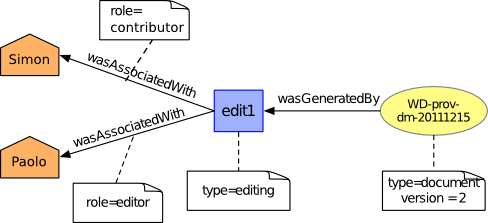
\includegraphics[width=.5\linewidth]{imgs/prov.PNG}
\end{figure}

\framebreak

Data quality
\i Monitoring of the quality (e.g., accuracy) of the objects produced
\i notify when a transformation pipeline is not behaving as expected

Debugging 
\i Inferring the cause of pipeline failures is challenging
\i Store inputs of each operation along with 
\si their versions
\si environmental settings (e.g., RAM and CPUs)

And so on...

\framebreak

Are we done? no!
\i metadata can become bigger than data themselves
\i we need meta meta-data (or models)...
\i ... chasing our own tails
\end{frame}

\sssec{From PaaS to FaaS (serverless)}
\begin{frame}[allowframebreaks]{From PaaS to FaaS (serverless)}

Cloud services are hosted in multiple locations worldwide
\i Locations are composed of regions and availability zones
\i Each region has multiple availability zones. 
\si Each region is a separate geographical area
\si Each region is completely independent
\si Availability zones in a region are connected through low-latency links
\si Resources are usually replicated across zones but not regions

\framebreak

%\begin{frame}{Types of cloud}
\begin{figure}
    \centering
    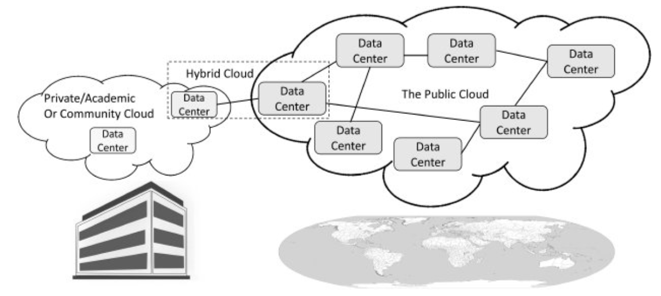
\includegraphics[height=.5\textheight]{imgs/cloud_types.png}
\end{figure}
\i Public: accessible to anyone willing to pay (e.g., Microsoft, AWS, Google)
\i Private: accessible by individuals within an institution
\i Hybrid: a mix of the previous

%\end{frame}
\framebreak
%\begin{frame}{Cloud providers}

\begin{figure}
    \centering
    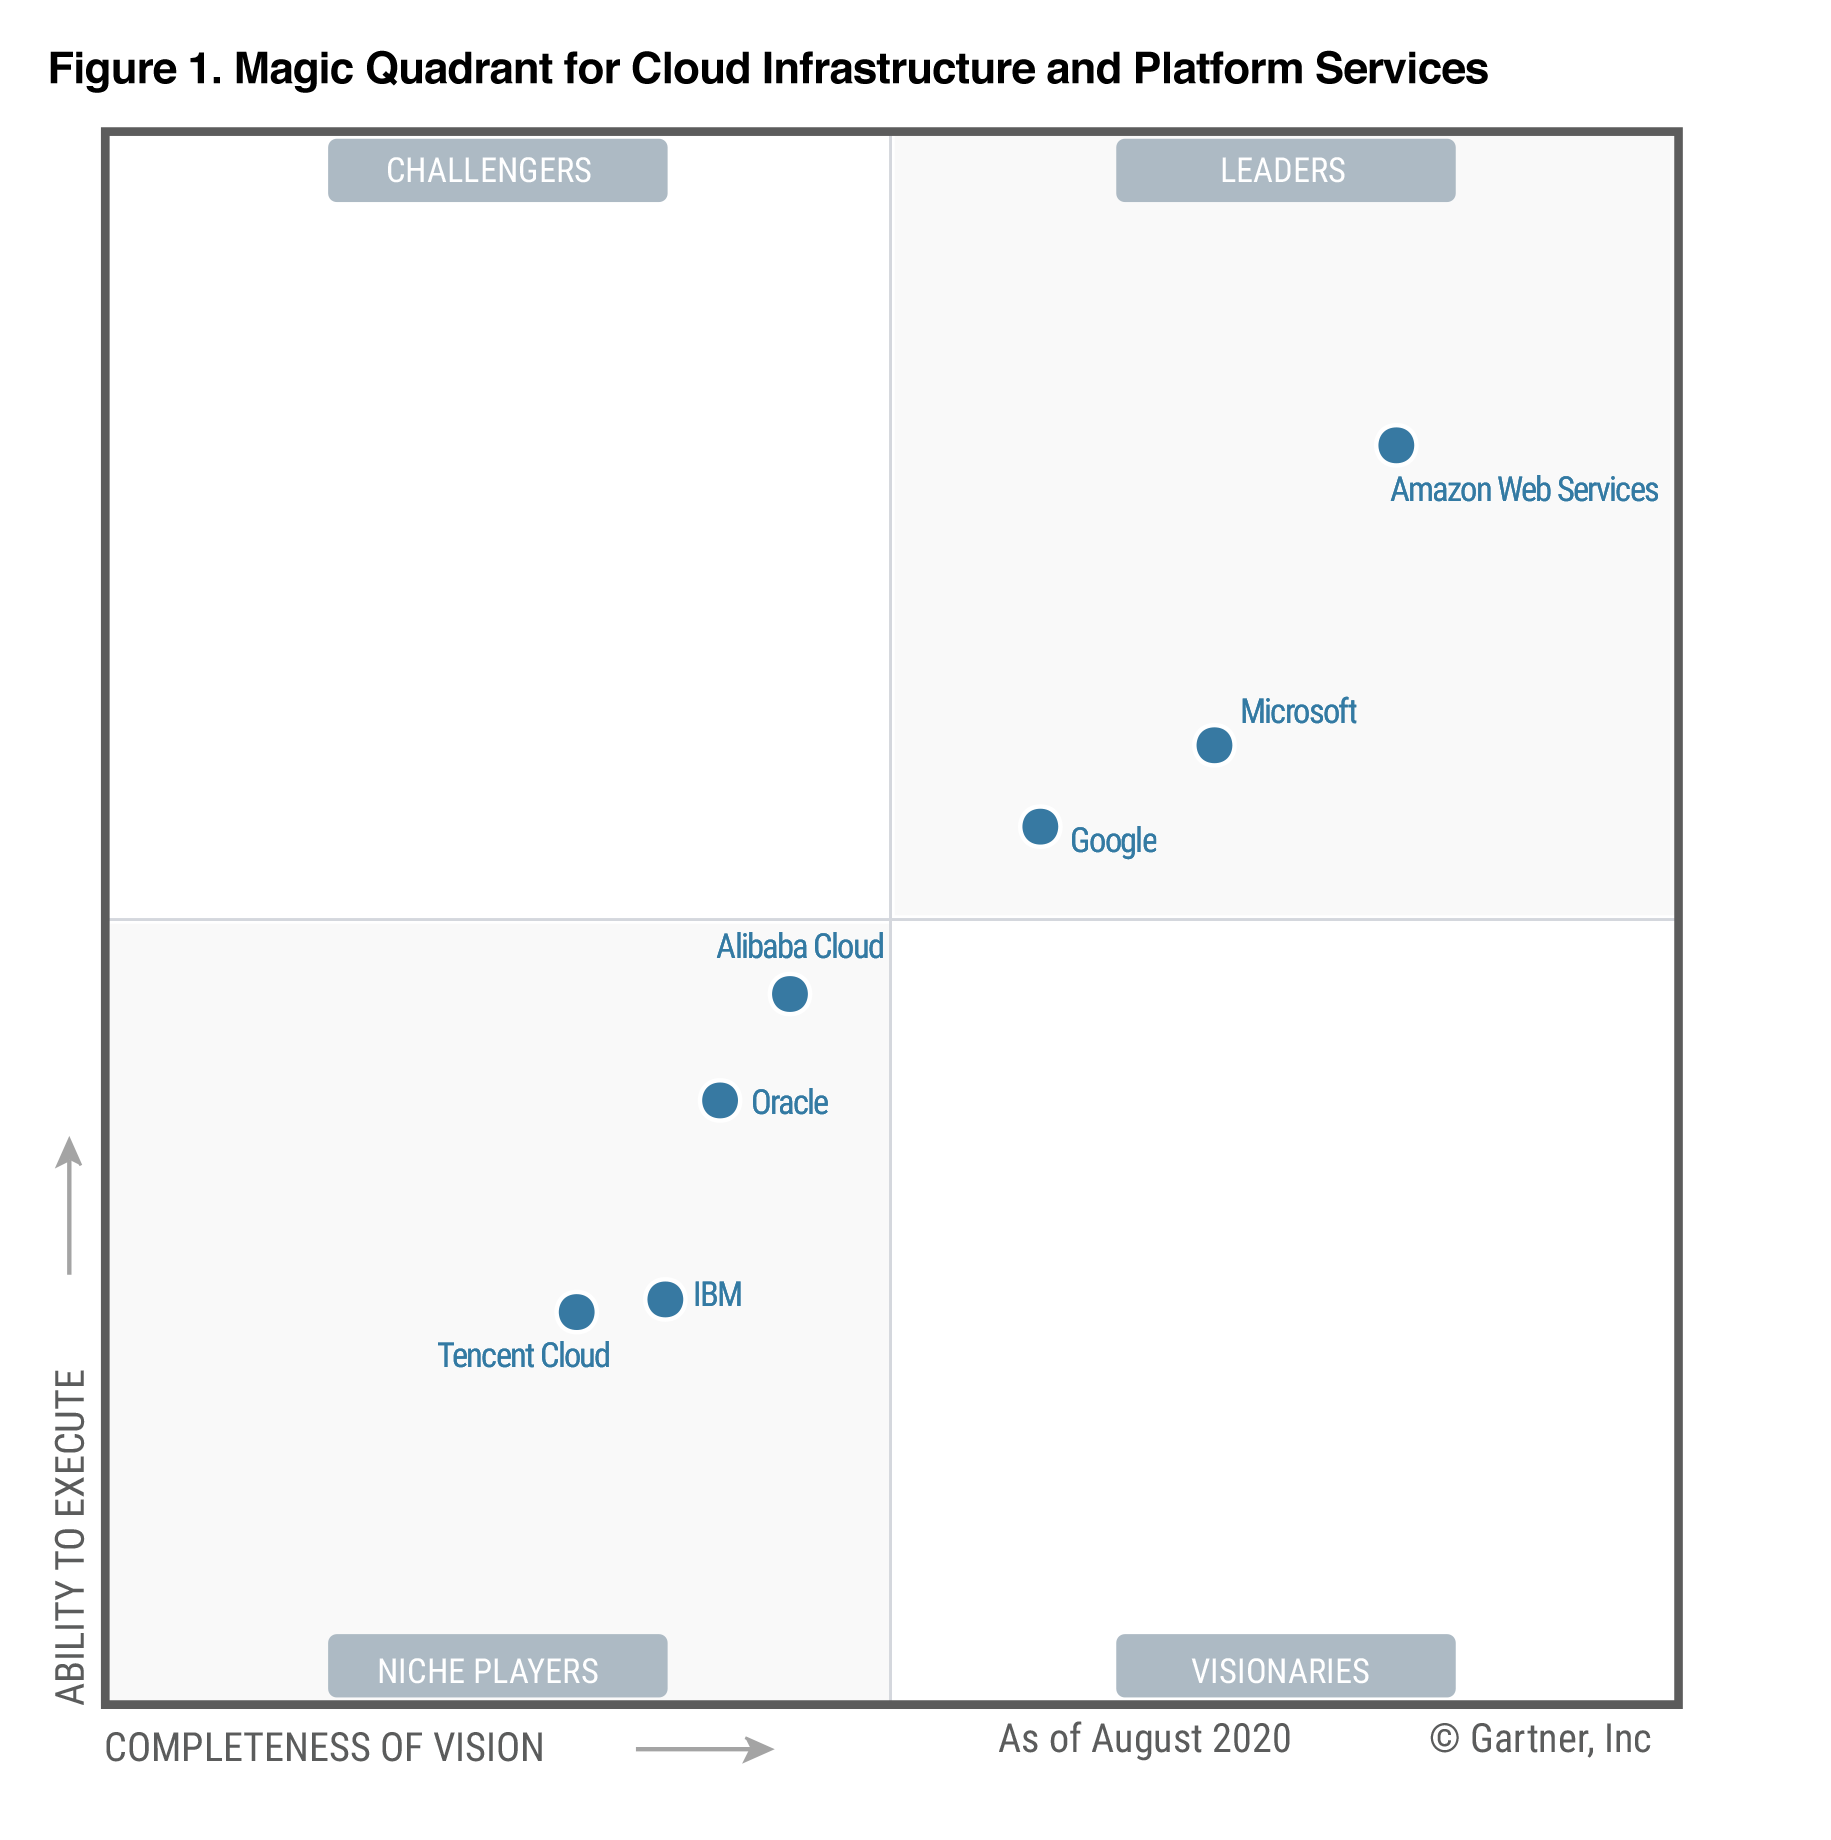
\includegraphics[height=.8\textheight]{imgs/cloud_providers.png}
\end{figure}

%\end{frame}
\framebreak
% \begin{frame}{Types of cloud}

\begin{figure}
    \centering
    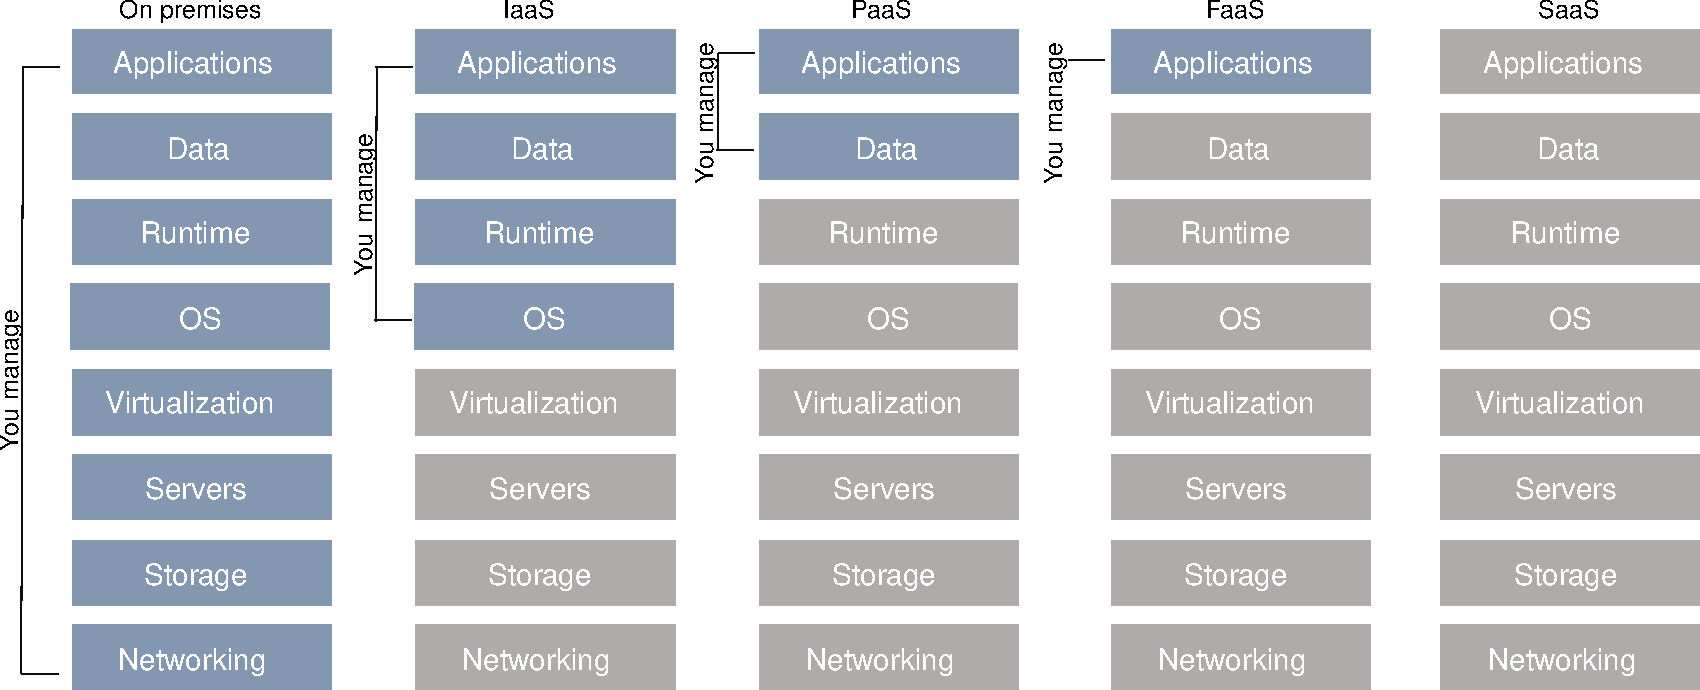
\includegraphics[height=.6\textheight]{imgs/cloud_paastosaas.pdf}
\end{figure}

%\end{frame}
\framebreak
%\begin{frame}[allowframebreaks]{Types of cloud}

Understanding architectures is paramount to successful software systems
\i good architectures help to scale
\i poor architectures cause issues that necessitate a costly rewrite

\textbf{On premises}
\i provisioning, managing, and patching servers is time-consuming
\i require dedicated operations people
\i a non-trivial environment is hard to set up and operate effectively
\i infrastructure and hardware are often a distraction from strategic tasks

\framebreak

\textbf{Infrastructure as a service (IaaS)} 
\i a computing infrastructure provisioned and managed over the internet
\i avoid expense/complexity of buying/managing \textit{physical} servers/data-centers
\i IaaS overcomes issues on premises
\si possibly requires to manage many environments

\textbf{Platform as a Service (Paas)}
\i a development and deployment environment in the cloud
% \i like IaaS, includes infrastructure-servers, storage, and networking
\i support complete application life-cycle: building, testing, deploying, etc.
\i avoid expense/complexity of managing licenses and application infrastructure

\framebreak

\textbf{Function as a Service (FaaS)}
\i a coding environment, cloud provider provisions platform to run the code
\i infrastructure provisioning and management are invisible to the developer
\i avoid to manage infrastructure

\textbf{Software as a service (SaaS)} 
\i an application environment 
\i access cloud-based apps over the Internet (e.g., email, Microsoft Office 365)
%\end{frame}
\framebreak
% \begin{frame}[allowframebreaks]{From PaaS to FaaS (serverless)}

\textbf{PaaS} and \textbf{containers} are potential solutions to inconsistent infrastructures

\i \textbf{PaaS} provides a platform for users to run their software
\si developers write software targeting features/capabilities of the platform

\i \textbf{containerization} isolates an application with its own environment
\si lightweight alternative to full virtualization
\si containers are isolated but need to be deployed to (public/private) server
\si excellent solution when dependencies are in play
\si "housekeeping" challenges and complexities

% \begin{block}{Microservices}
% Small, standalone, fully independent services built for a specific purpose
% \end{block}
% \i Each service written in an appropriate framework and language
% \si Benefits from the right language/libraries
% \si Many languages and frameworks are hard to support
% \i Each microservice can maintain state and store data
% \si eventual consistency, transaction management, and complex error recovery can make things hard

\framebreak


\textbf{Serverless}
\i a software architecture that does not rely on direct access to a server

FaaS is based on a serverless approach
\i every function could be considered as a standalone service
\i embodies principles from microservices
\si small, standalone, fully independent services built for a specific purpose
\si each service written in an appropriate framework and language
\i cloud provider is responsible for integration 
% \i Many languages and frameworks are hard to support
% \i Each microservice can maintain state and store data

\framebreak

Principles of FaaS/serverless architectures
\i use a compute service to execute code on demand (no servers/containers)
\i write single-purpose stateless functions
\i functions react to events
\si design push-based, event-driven pipelines
\i create thicker, more powerful front ends
\i embrace third-party services
\i security is designed for each function

\framebreak

Write single-purpose stateless functions
\i keep the single responsibility principle in mind
\si a function that does just one thing is more testable and robust
\si a function with a well-defined interface is also more likely to be reused
\i code should be created in a stateless style
\si local resources or processes will not survive along sessions
\si statelessness allows scalability
\i functions that terminate sooner are cheaper 
\si (pricing is based on \#requests, execution time, and allocated memory)
% Having less to do in Lambda is cheaper.  Moreover, building a rich front end (in lieu of a complex back end) that can talk to third-party services directly can be conducive to a better user experience. Fewer hops between online resources and reduced latency will result in a better perception of performance and usability of the application. In other words, you don’t have to route everything through a compute service. Your front end may be able to communicate directly with a search provider, a database, or another useful API.

Compose functions in a loose orchestration
\i build complex but understandable back-end systems
\i event-driven and push-based pipelines

\framebreak

FaaS/Serverless is not a silver bullet
\i not appropriate for latency-sensitive applications 
\i strict specific service-level agreements
\i vendor lock-in can be an issue for enterprise and government clients
\i should not base mission-critical applications on a public cloud
\i Lock-in issues
\i Migration

% TODO: Migration to cloud: pattern prevedibile? carico di lavoro? quantità dati? CPU? RAM? sposto tutto AS IS? Oppure posso ottimizzare? EMR (cluster EC2 vs cluster Kubernetes). Gestito = sicurezza + isntallazione + monitoring, logging

\end{frame}

% \begin{frame}{History in (very) brief}
% Computing as a service is far from new

% \begin{itemize}
% \item 1961, John McCarthy at MIT: "Computing may someday be organized as a public utility just as the telephone system [...] Each subscriber needs to pay only for the capacity he uses, but he has access to all programming languages characteristic of a very large system" 
% \item 1969, UCLA turns on first node of ARPANET. "As [computer networks] grow up and become more sophisticated, computer utilities will spread"
% \item 1990s USA, gigabit testbeds linked research laboratories. "Meta-computer", virtual computational systems created by linking components at different sites
% \item Large Hadron Collider (LHC) federates computing systems at hundreds of sites to analyze PBs of data. LHC Computing Grid enables on-demand access to computing and storage 
% % 2006 Emergence of cloud computing, a story of marketing, business model, and technological innovation
% % \i Cloud is driven by a transformation in demand (First successful IaaS emerged from an e-commerce provider)
% % \i Amazon was building hundreds of similar work-unit computing systems to support different services
% \end{itemize}
% \end{frame}
% \begin{frame}{Data transformation}
% 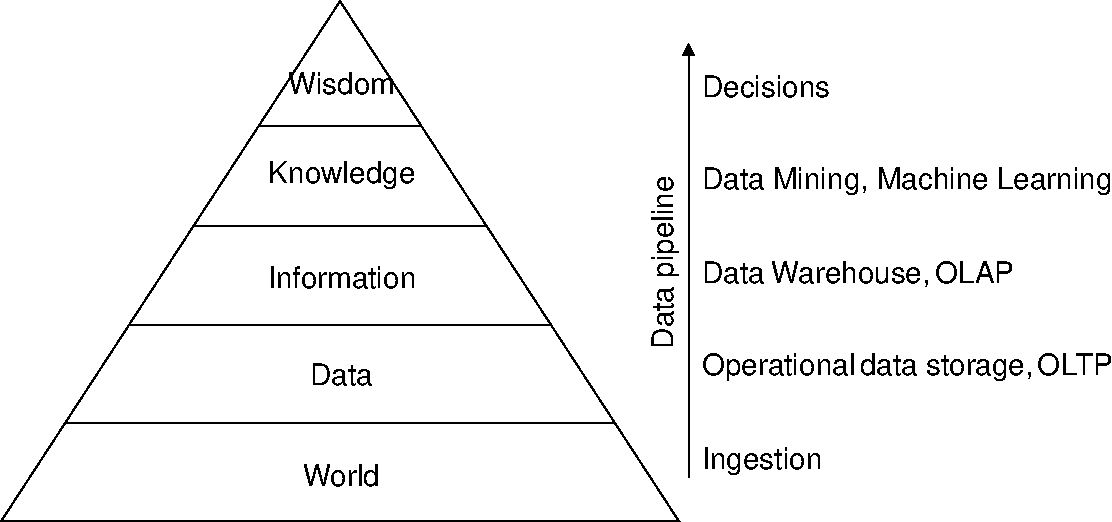
\includegraphics[height=.8\textheight]{imgs/knowledgepyramid.pdf}
% \end{frame}


\ssec{Data pipelines on cloud}

\begin{frame}{}

\includegraphics[width=\linewidth]{imgs/xkcd_pipeline.png}    
\end{frame}

\begin{frame}{Date pipelines on cloud}
Architecting data pipelines on cloud requires to \textbf{standardize/integrate} services
\i Make them available through simple portals
\i Track usage/cost with billing mechanism
\i Measure availability
\i Orchestrate to meet demand
\i Provide a security framework
\end{frame}

\begin{frame}{Which services do we need?}
\begin{figure}
\centering
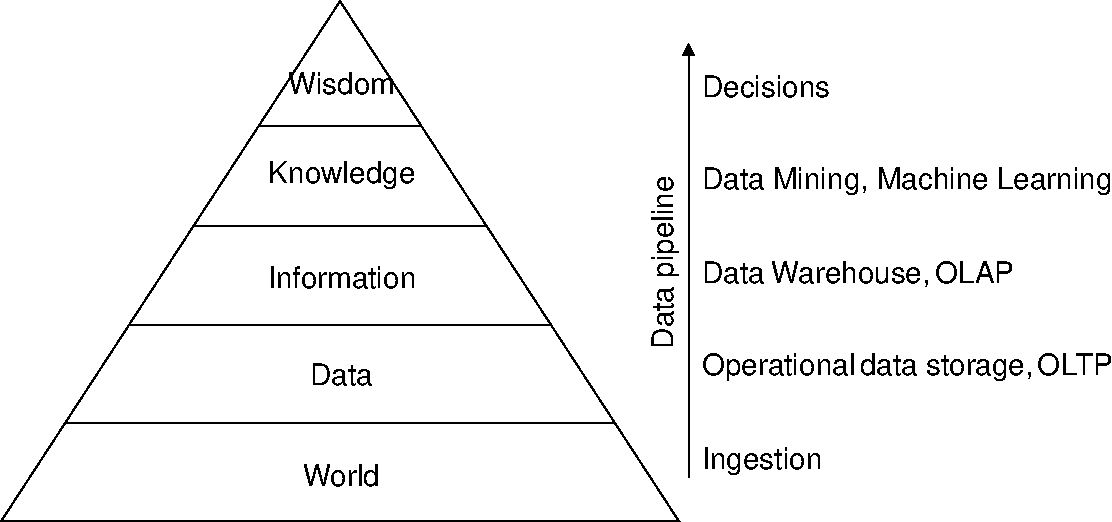
\includegraphics[height=.7\textheight]{imgs/knowledgepyramid.pdf}
\end{figure}
\end{frame}

\begin{frame}[allowframebreaks]{A tentative organization}
\begin{figure}
\centering
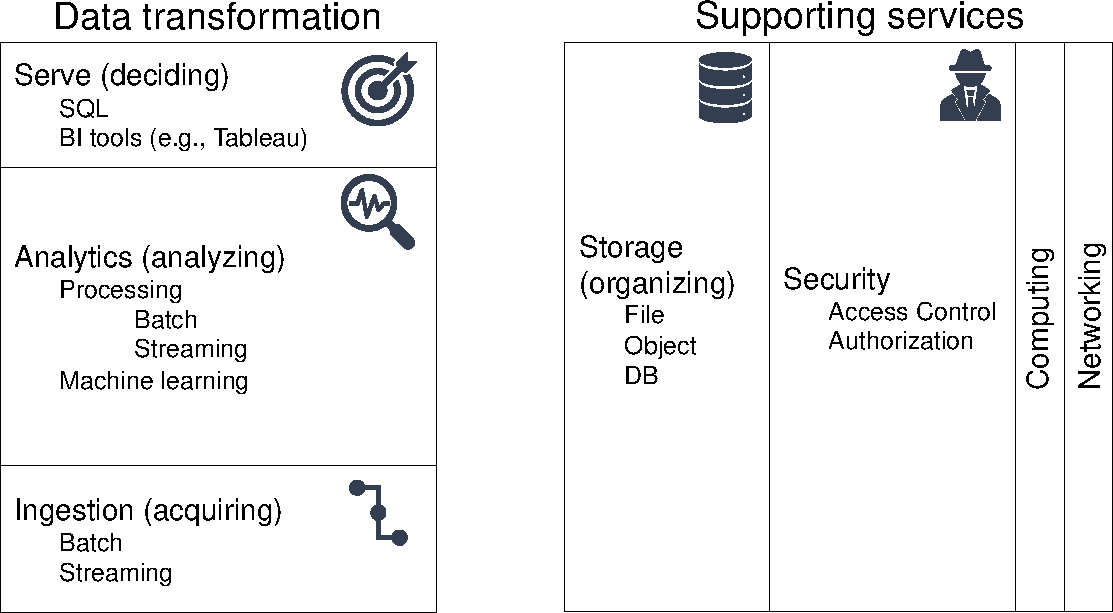
\includegraphics[height=.7\textheight]{imgs/cloudpatchwork.pdf}
\end{figure}

\framebreak

Not a sharp taxonomy

Ingestion vs Analytics
\i Data streams are used for ingestion
\i ... and (event) processing

Storage vs Database 
\i Databases are storage
\i ... with processing capability
\i ... and with serving capability

\framebreak

Categorizing features (the big-data cube \cite{meijer2012your})
\begin{columns}
\begin{column}{0.5\textwidth}
\begin{itemize}
\item Volume: small to high
\item Variety: structure to unstructured
\item Velocity: pull to push
\end{itemize}
\end{column}
\begin{column}{0.5\textwidth}
\begin{figure}
\centering
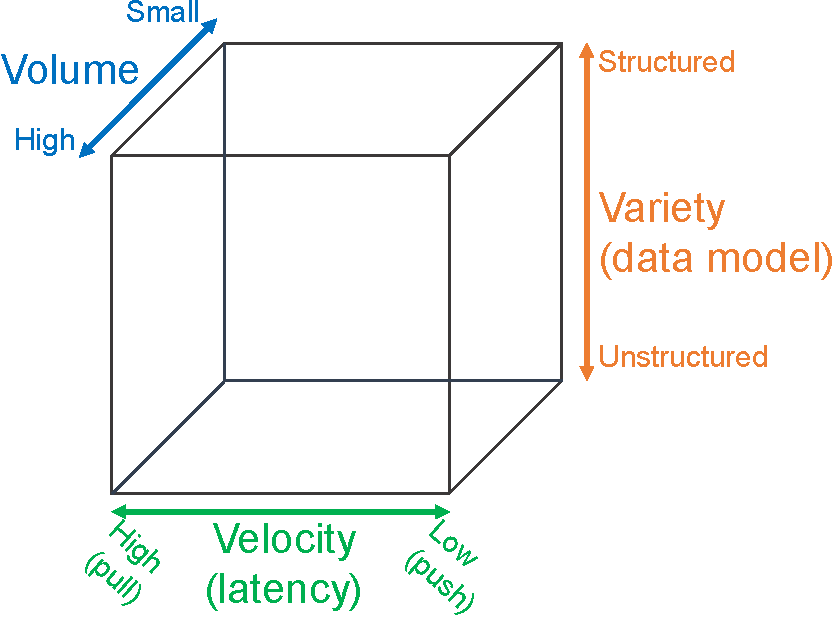
\includegraphics[scale=.4]{imgs/bigdatacube.pdf}
\end{figure}
\end{column}
\end{columns}

\framebreak

\begin{columns}
\begin{column}{0.5\textwidth}
Volume
\begin{itemize}
\item Small: small relational DBs
\item High: TBs o PBs of data
\end{itemize}
\end{column}
\begin{column}{0.5\textwidth}
\begin{figure}
\centering
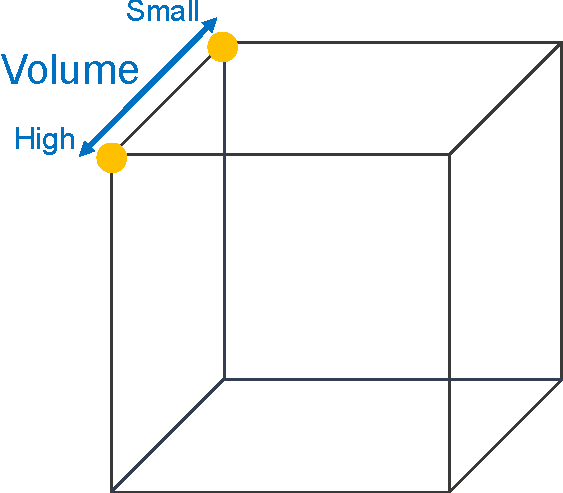
\includegraphics[scale=.4]{imgs/bigdatacube1.pdf}
\end{figure}
\end{column}
\end{columns}

\framebreak

\begin{columns}
\begin{column}{0.5\textwidth}
Variety
\begin{itemize}
\item structured: relational tuples with FK/PK relationships
\item unstructured
\begin{itemize}
    \item key-value
    \item columnar
    \item document-based
    \item graph
\end{itemize}
\end{itemize}
\end{column}
\begin{column}{0.5\textwidth}
\begin{figure}
\centering
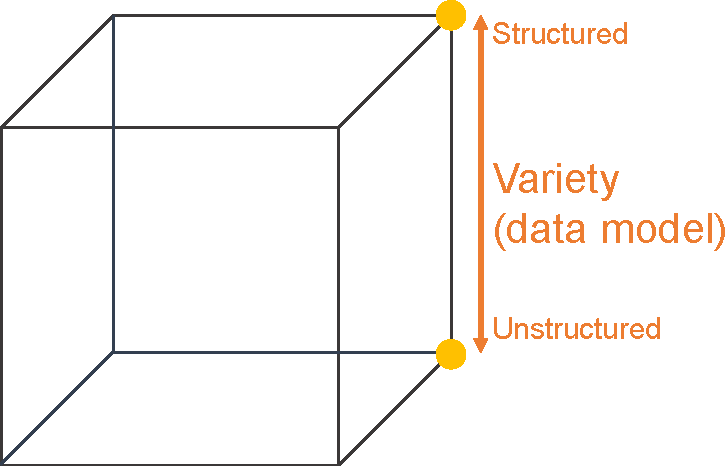
\includegraphics[scale=.4]{imgs/bigdatacube2.pdf}
\end{figure}
\end{column}
\end{columns}

\framebreak

\begin{columns}
\begin{column}{0.5\textwidth}
Velocity (latency)
\begin{itemize}
\item high: clients synchronously pulling data from sources 
\item low: sources asynchronously pushing data to clients
\end{itemize}
\end{column}
\begin{column}{0.5\textwidth}
\begin{figure}
\centering
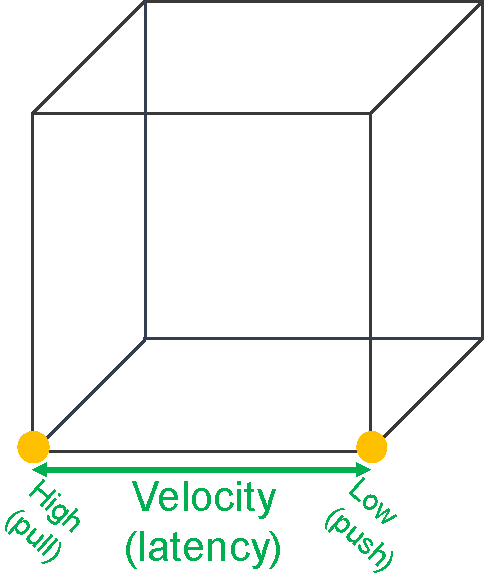
\includegraphics[scale=.4]{imgs/bigdatacube3.pdf}
\end{figure}
\end{column}
\end{columns}

\framebreak

\begin{columns}
\begin{column}{0.5\textwidth}
Our focus (in this course)
\begin{itemize}
\item (un)structured big-data batch
\item (un)structured big-data streams
\end{itemize}

\textbf{Goal}: keep in mind the cube to categorize the following services
\end{column}
\begin{column}{0.5\textwidth}
\begin{figure}
\centering
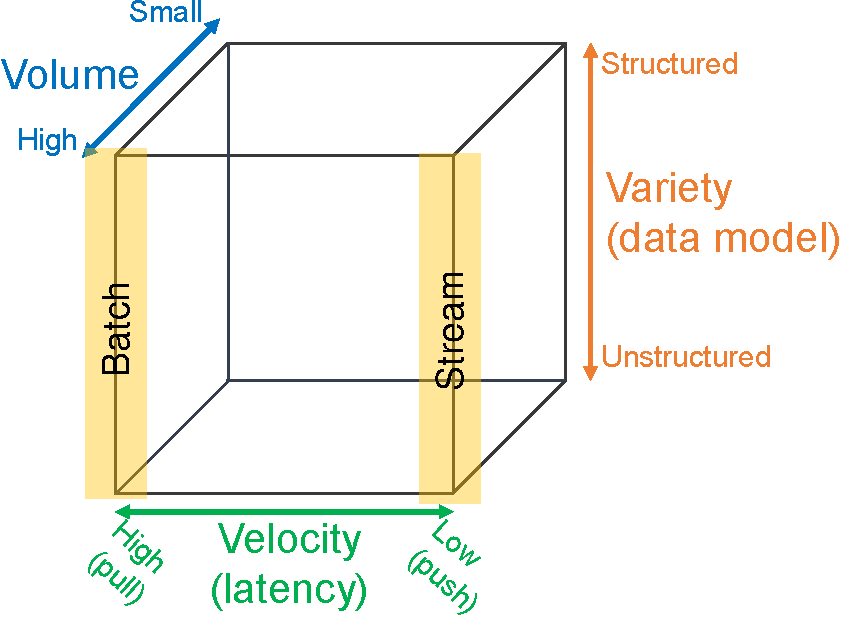
\includegraphics[scale=.4]{imgs/bigdatacube4.pdf}
\end{figure}
\end{column}
\end{columns}

% \framebreak

% \begin{figure}
%     \centering
%     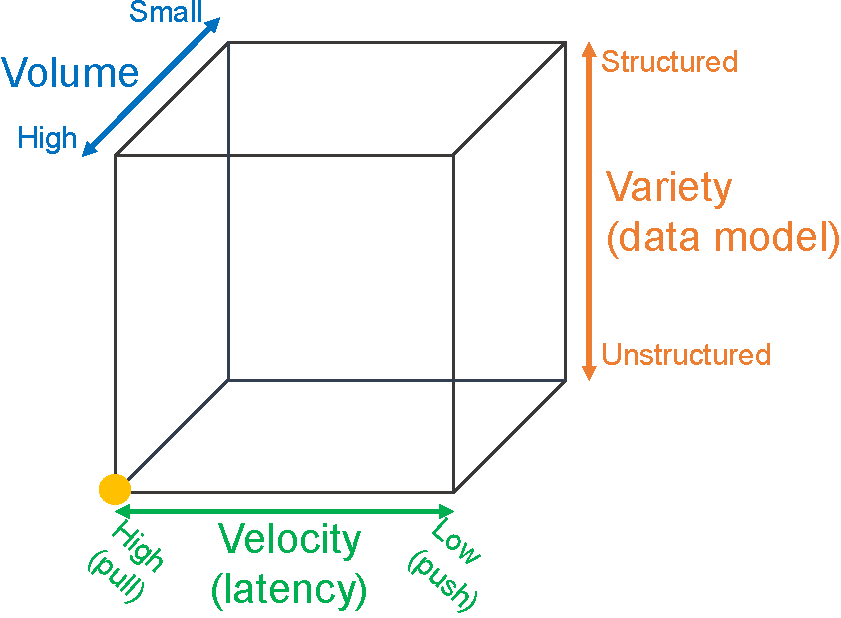
\includegraphics[scale=.4]{imgs/bigdatacube5.pdf}
% \end{figure}

% \framebreak

% \begin{figure}
%     \centering
%     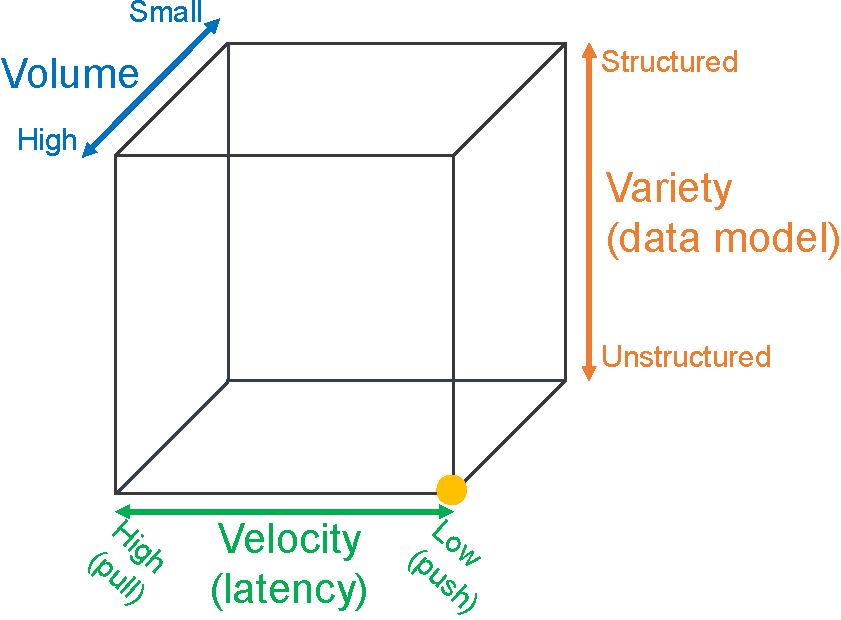
\includegraphics[scale=.4]{imgs/bigdatacube6.pdf}
% \end{figure}

% \begin{frame}[allowframebreaks]{At what costs?}
% Physical costs (and economy of scale)
% \si charges for AWS have been reduced 42 times since 2008 (up to 2014)
% \si 12/2014, charges for outbound data transfer were lowered by up to 43\%
% \si 11/2014, charges for search service were lowered by 50\%
% \si 03/2014, charges for virtual server were lowered by up to 40\%


% However, datasets are
% \i From various sources and unstructured (variety) 
% \i Of large size (volume)
% \i With fast data in/out (velocity)

% \textbf{Challenges}: data assimilation, aggregation, classification, etc.
% \end{frame}


% \begin{frame}{Data pipeline on cloud: AWS}
% \url{https://aws.amazon.com/it/architecture/analytics-big-data}
\framebreak

AWS

\begin{figure}
    \centering
    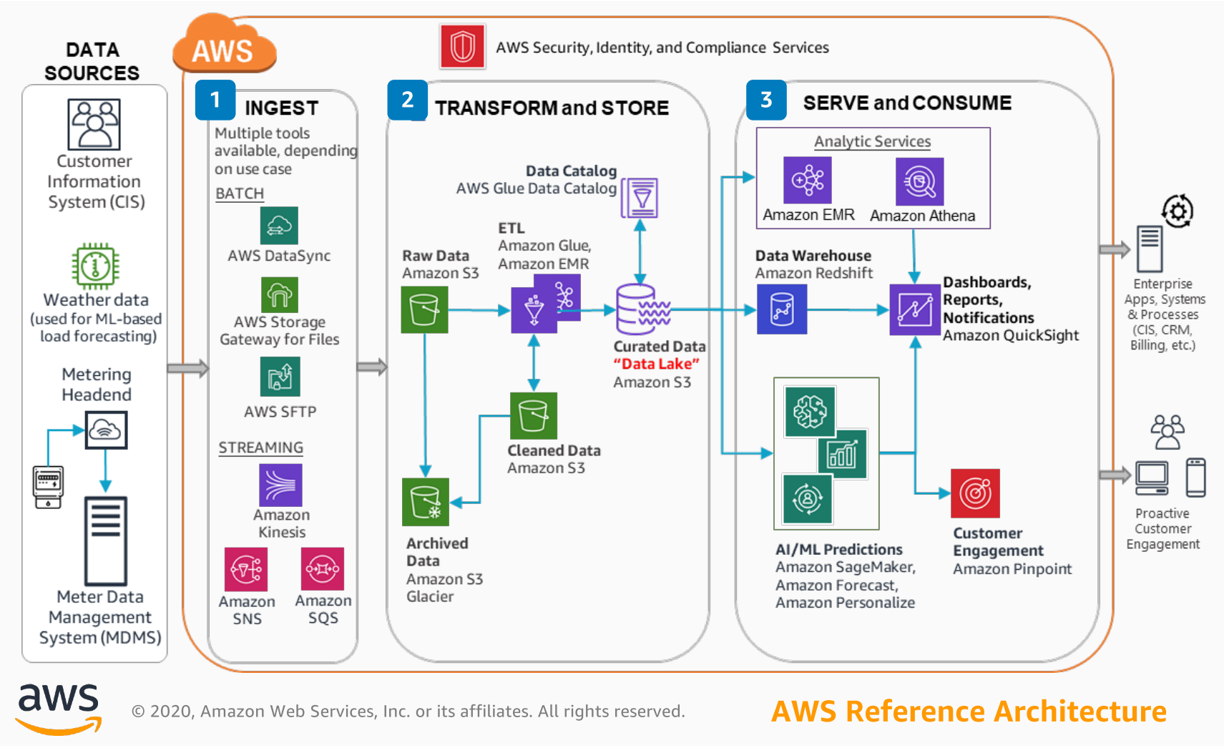
\includegraphics[height=.7\textheight]{imgs/awspipeline.png}
\end{figure}
% \end{frame}
% \begin{frame}[allowframebreaks]{AWS: storage}\end{frame}

\framebreak

% \begin{frame}{Data pipeline on cloud: Google Cloud}
Google cloud 

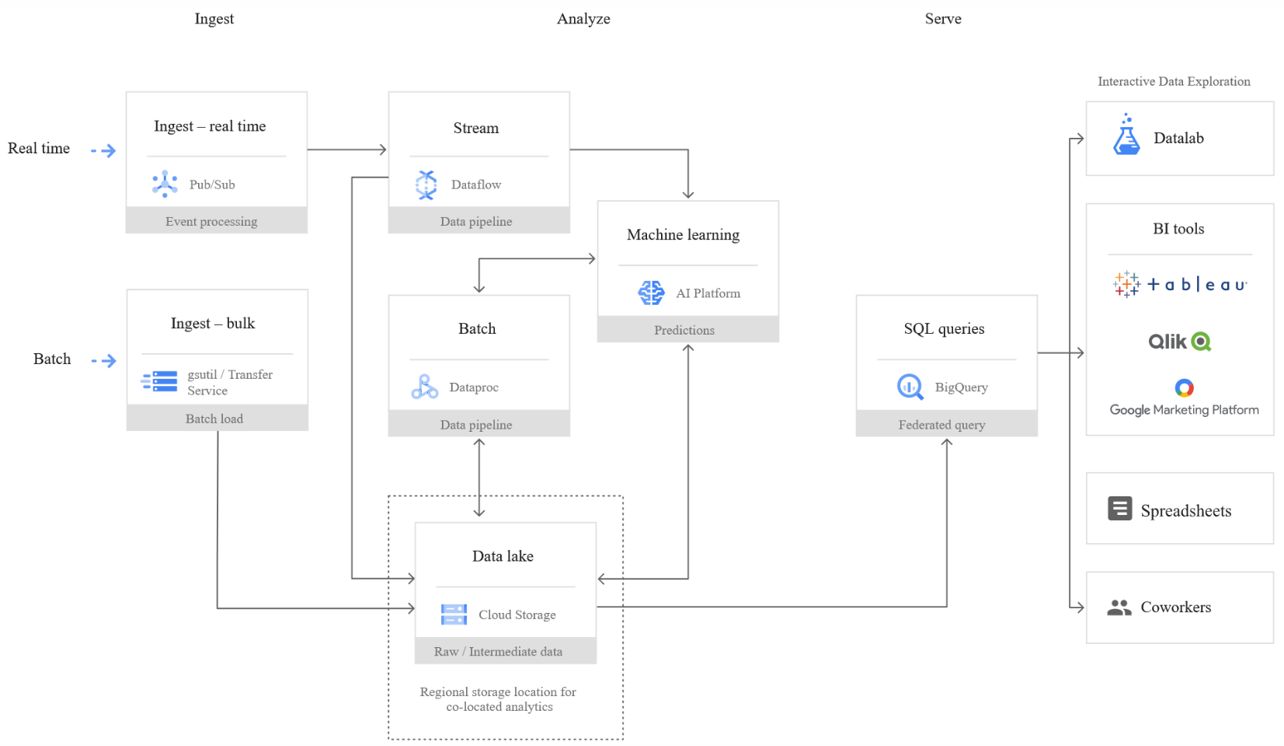
\includegraphics[height=.7\textheight]{imgs/gcpipeline.png}

% AI services: pre-trained models accessible through API (e.g., transcribe)
% ML services: sagemaker, helping in training models
% Or, "low-level" frameworks (e.g., TensorFlow)
\end{frame}

\sssec{Storage}
\begin{frame}[allowframebreaks]{Storage}
\textbf{Goal}: persisting data

\textbf{Storage models}
\i Different ways in which data are organized in a storage system

Understand different storage models to choose the right one
\i Nature and size of the data
\i Analyses to be performed
\i Access/update frequencies

\framebreak
% \end{frame}

% \begin{frame}[allowframebreaks]{Storage: types of storage models}

\textbf{File system} 
\i stores unstructured binary objects in a tree of directories (folders)
\i + extremely intuitive storage abstraction
\i - no support for representing structured data
\i - hierarchical organization could not match relationships
\i - cannot navigate complex data collections
\i - need to maintain consistency as multiple processes read/write a file system

\framebreak
Amazon EFS
\i deploy FS within a specific region
\i amazon EC2 instances within that region can access that file system
\i with amazon vpc/direct connect, mount file system to on-premises machine
\i cost
\si priced by average number of gb used per month
\si if provisioned throughput, also charged by provisioned mb of throughput
\si pricing also varies according to the region

\framebreak
Google Filestore
\i deploy instances within a specific zone
\i mount fs instance in any computing instance as long as in the same network
\i cost
\si priced by gbps and by service tier (standard or premium)
\si varies according to the region

\framebreak
\begin{table}
\centering
\footnotesize
\begin{tabular}{lp{5cm}p{5cm}}
    \multicolumn{1}{c}{\textbf{Feature}} & \multicolumn{1}{c}{\textbf{Amazon EFS}} & \multicolumn{1}{c}{\textbf{Filestore}} \\
    \midrule
    Tiers/Modes & General Purpose and Max I/O. Each supports either Bursting Throughput or Provisioned Throughput mode. & Standard and premium \\
    Deployment locality & Regional & Zonal \\
    Protocol & NFSv4 & NFSv3 \\
    Encryption & Can be enabled at rest and in transit & By default, encrypted at rest and in transit \\
    Pricing & Priced by average number of GB used per month and by region of deployment. If using Provisioned Throughput mode, also priced by provisioned MB of throughput. & Priced per allocated GB per second, by region of deployment, and by service tier. \\
\end{tabular}%
\end{table}%

\framebreak

\textbf{Object Store}
\i stores unstructured binary objects (blobs, binary large object)
\i simplifies the file system model, in general supports a two-level hierarchy
\i + eliminates hierarchy 
\i + forbids updates to objects once created
\i - little support for organizing data and no support for search
\i - user must know an object's identifier to access it

\framebreak
Cloud Storage and Amazon S3
\i store objects in a bucket
\i Each object within a bucket is identified by a unique key within that bucket
\i each object has an associated metadata record
\si object size, date of last modification, and media type
\si metadata can be modified
\si add custom metadata
\i user experience for buckets is designed to be similar to that of FS
\si object keys are usually paths such as ``/foo/subdir/baz.txt''
\si provide filesystem-like APIs—for example, e.g., ``ls -R''

\framebreak
\begin{table}
  \centering
  \footnotesize
    \begin{tabular}{lp{5cm}p{5cm}}
    \textbf{Feature} & \textbf{Amazon S3} & \textbf{Cloud Storage} \\
    Unit of deployment & Bucket & Bucket \\
    Deployment identifier & Globally unique key & Globally unique key \\
    File system emulation & Limited & Limited \\
    Obj. metadata & Yes   & Yes \\
    Obj. versioning & Yes   & Yes \\
    Update notifications & Event notifications & Pub/Sub notifications for Cloud Storage, Cloud Storage triggers for Cloud Functions, and object change notifications \\
    Service classes & Standard, Standard-Infrequent Access, One Zone-Infrequent Access, Amazon Glacier* & Standard, Nearline, Coldline, Archive \\
    Deployment locality & Regional & Multi-regional and regional \\
    Pricing & Priced by amount of data stored per month, network egress, and number of common API requests & Priced by amount of data stored per month, network egress, and number of common API requests \\
    \end{tabular}%
\end{table}%

\framebreak

Access frequency/retention determine availability and pricing
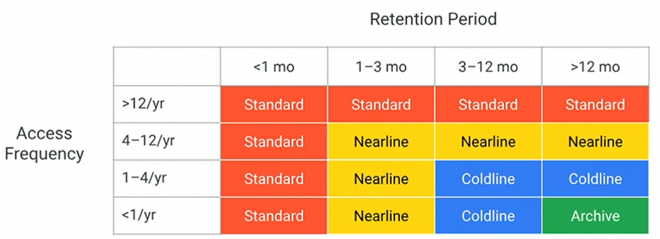
\includegraphics[width=.6\linewidth]{imgs/gc_accessfrequency.png}
\i Standard: optimized for performance and high frequency access
\i Nearline: for data accessed less than once a month
\i Coldline: for data accessed less than once a quarter
\i Archive: most cost-effective, data accessed less than once a year

\framebreak
Amazon Glacier
\i Cost
\si Amount of data stored per month
\si Size of files stored
\si Retrieval type
\si Number of retrieval requests
\si Network egress
\si Storage region
\i If you delete/modify data before the minimum storage period
\si charged for the remainder of the period
\si delete an object 5 days after storing the object, charged for remaining 85

\framebreak
Cloud Storage Archive
\i Cost
\si priced by amount of data stored per month and by network egress
\si Pricing also varies by storage region
\i If you delete/modify data before the minimum storage period
\si charged for the remainder of the period

% Table generated by Excel2LaTeX from sheet 'Sheet1'
\begin{table}
  \centering
  \footnotesize
    \begin{tabular}{lp{5cm}p{5cm}}
    \textbf{First-byte latency} & \textbf{Minutes to hours} & \textbf{Milliseconds (identical to Cloud Storage Standard)} \\
    \midrule
    Retrieval types & Expedited, Standard, Bulk. Expedited users can also choose between On-Demand or Provisioned retrieval. & N/A \\
    Deployment locality & Regional & Multi-regional or regional \\
    Minimum storage period & 90 days & 365 days \\
    SLA   & No    & No \\
    Pricing & Priced by amount of data stored per month, size of files stored, retrieval type, number of retrieval requests, network egress, storage region, storage period, and number of common API requests & Priced by amount of data stored per month, network egress, storage region, storage period, and number of common API requests \\
    \end{tabular}%
\end{table}%

\textbf{Database} 
\i relational
\i NoSQL
\si key-value
\si columnar
\si document based
\si graph

\framebreak
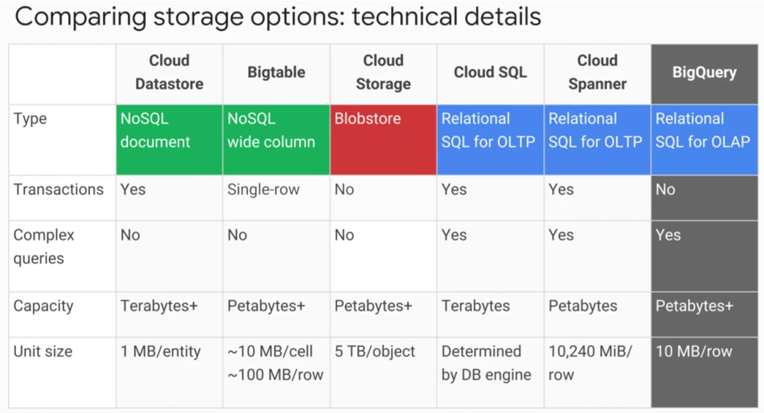
\includegraphics[width=.8\linewidth]{imgs/gc_storage_analyses.png}

\framebreak
\begin{table}
    \footnotesize
    \centering
    \begin{tabular}{lp{5cm}p{5cm}} %p{3cm}
        \textbf{Model} & \textbf{Amazon}                                   & \textbf{Google}                        \\\hline%& \textbf{Azure} \\\hline
        Files       & Elastic File System (EFS), Elastic Block Store (EBS) & Google file system                     \\%& Azure File Storage  \\
        Objects     & Simple Storage Service (S3)                          & Cloud Storage                          \\%& Blob Storage Service\\
        Relational  & Relational Data Service (RDS), Aurora                & Cloud SQL, Spanner                     \\%& Azure SQL           \\
        NoSQL       & DynamoDB, HBase                                      & Cloud Datastore, Bigtable              \\%& Azure Tables, HBase \\
        Graph       & Titan                                                & Cayley                                 \\%& Graph Engine        \\
        Warehouse   & Redshift                                             & BigQuery                               \\%& Data Lake           \\
    \end{tabular}
\end{table}
\end{frame}

\sssec{Ingestion}
\begin{frame}[allowframebreaks]{Ingestion}
\textbf{Goal}: moving data to the cloud

Ingestion services, which are used to ingest data from a source environment into a reliable and stable target environment or data type.

Moving data to the cloud
\i \r{80TB} of data to move, \g{1Gbps} connection to the internet
\i \b{How many days}? 
\si \r{80000GB} / \g{(1Gbps / 8)} / \b{60 / 60 / 24} \~= a week without internet

\framebreak
\textbf{Batch/Bulk}
\i Move data from on-premises storage

Workflow 
\i receive shipment
\i set up
\i  transfer data
\i ship back ( shipping carrier)

\framebreak
AWS Snowball
\i AWS Snowball comes in 50TB (North America only) and 80TB versions
\i AWS Snowball is not rack-mountable
\i Throughput
\si 1 Gbps or 10 Gbps using an RJ-45 connection
\si 10 Gbps using a fiber optic connection

\framebreak
Google Transfer Appliance
\i 100TB version known as the TA100, 480TB version known as the TA480	
\i TA100 comes in a 2U rack-mountable, TA480 is not rack-mountable
\i Throughput
\si 1 Gbps or 10 Gbps using an RJ-45 connection
\si 10 Gbps using a fiber optic connection
\si 4 ethernet ports, adaptive load balancing for multi-stream throughput

\framebreak
\begin{table}
  \centering
  \footnotesize
    \begin{tabular}{lll}
    \textbf{Feature} & \textbf{AWS Snowball} & \textbf{Transfer Appliance} \\
    \midrule
    Capacity per unit & 50 TB or 80 TB & 100 TB or 480 TB \\
    \multirow{3}[0]{*}{Maximum transfer rate} & \multirow{3}[0]{*}{10Gbps} & 20Gbps for TA100 \\
    \multicolumn{1}{l}{} & \multicolumn{1}{l}{} & 40Gbps for TA480 \\
    \multicolumn{1}{l}{} & \multicolumn{1}{l}{} & Both with automatic link aggregation \\
    Email status updates? & No    & Yes \\
    \multirow{2}[0]{*}{Rack-mountable?} & \multirow{2}[0]{*}{No} & Yes for TA100 \\
    \multicolumn{1}{l}{} & \multicolumn{1}{l}{} & No for TA480 \\
    \multirow{2}[0]{*}{Use fee} & \$200 for 50 TB & \$300 for TA100 \\
    \multicolumn{1}{l}{} & \$250 for 80 TB & \$1800 for TA480 \\
    \multirow{2}[0]{*}{Daily fee} & \multirow{2}[0]{*}{\$15/day after 10 days} & \$30/day after 10 days for TA100 \\
    \multicolumn{1}{l}{} & \multicolumn{1}{l}{} & \$90/day after 25 days for TA480 \\
    Transfer modes & Push  & Push or pull \\
    Transfer data out of object store? & Yes   & No \\
    \end{tabular}%
\end{table}%

\framebreak
\textbf{Stream}
\i Real-time streaming data 

% \ssec{Event streams}
% \begin{frame}{Key concepts}

\textbf{Event}: anything that we can observe occurring at a particular point in time

\textbf{Continuous streaming}: an illimitated succession of individual events, ordered by the point in time at which each event occurred

\textbf{Publish/subscribe (pub/sub)}: a way of communicating messages

\i Senders publish messages associated with one or more topics
\i Receivers subscribe to specific topics, receive all messages with that topic
\i Messages are events
% \end{frame}

\framebreak
% \begin{frame}{The unified log}

\begin{block}{Unified log}

Unified, append-only, ordered, distributed log that allows the centralization of continuous event streams

\end{block}

General idea:

\i Collect events from disparate source systems
\i Store them in a unified log
\i Enable data processing applications to operate on these event streams
% \end{frame}

\framebreak
% \begin{frame}{Features of a unified log}

\textbf{Unified}: a single deployment of this technology a company, with multiple applications sending events to it and reading events from it
  \i Log serves as central data backbone
  \i Unified log can contain many distinct continuous streams of events
  \si Not all events are sent to the same event stream

\textbf{Append-only}: new events are appended to the unified log
\i existing events are never updated in place
\i if read the event \#10, never look at events 1 through 10 again
\i Events are automatically deleted from the unified log when they age 
% \end{frame}

\framebreak
% \begin{frame}{Features of a unified log}
\textbf{Distributed}: the unified log lives across a cluster of machines

\i Still, the log is unified since we have a single (conceptual)
\i Scalability: work with streams larger than the capacity of single machines
\i Durability: replicate all events within the cluster to overcome data loss
\i Divide events in a given stream into *shards* (partitions)

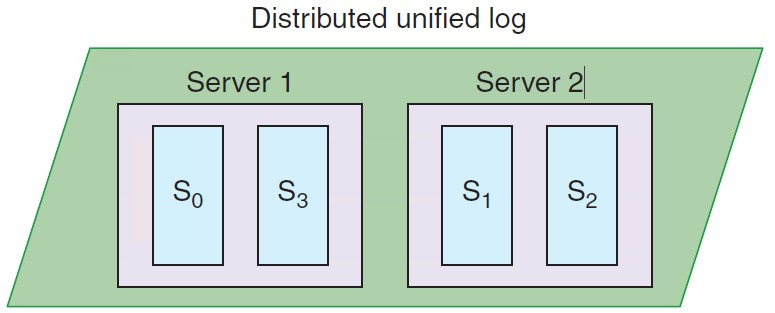
\includegraphics[width=.6\linewidth]{imgs/eventstream_shard.jpg}
% \end{frame}

% \begin{frame}{Features of a unified log}
\textbf{Ordered}: events in a shard have a sequential IDs (\textit{offset}, unique within a shard)
\i Local ordering keeps things much simpler
\i Applications maintain their own cursor for each shard

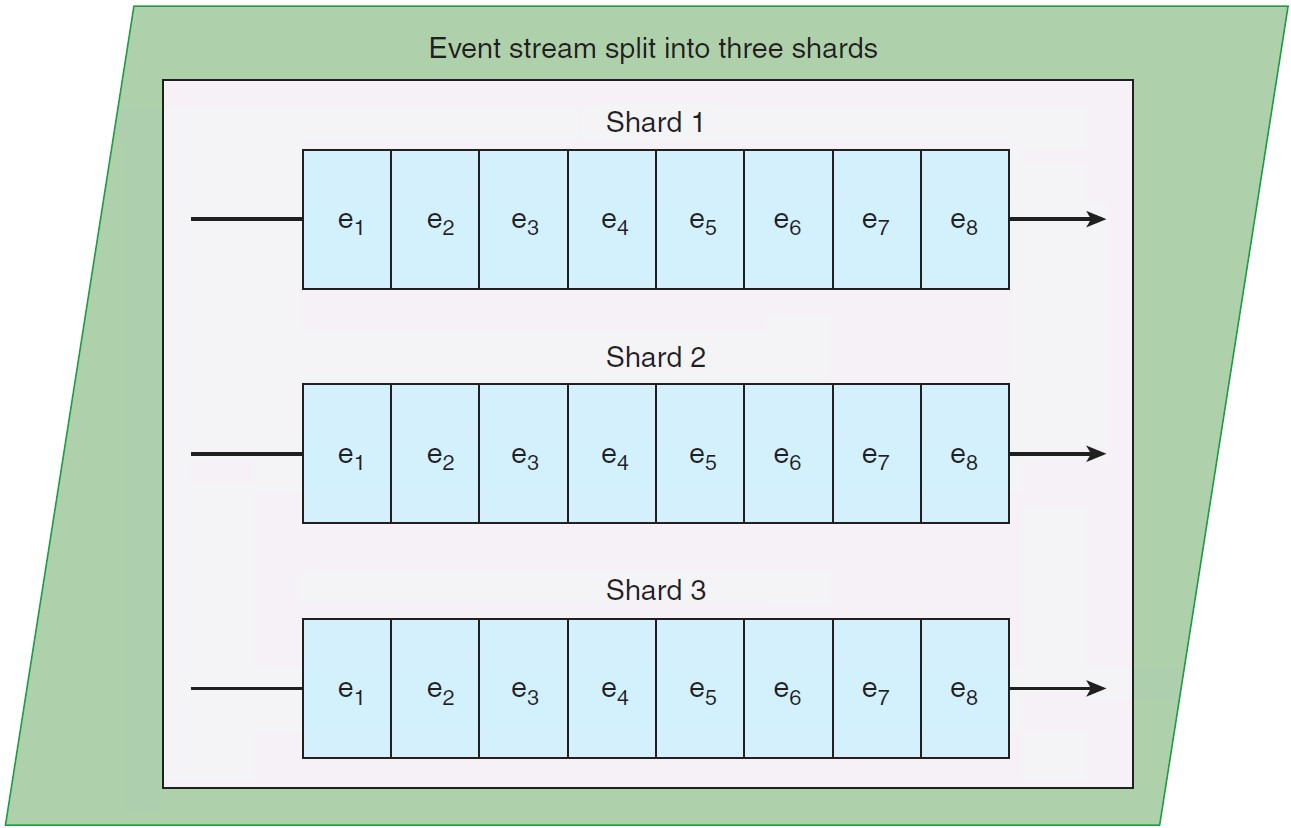
\includegraphics[width=.4\linewidth]{imgs/eventstream_order.jpg}
% \end{frame}

\framebreak
% \begin{frame}[allowframebreaks]{Event stream processing}
Two types of processing can be performed on a single event stream
\i \textbf{Single-event}, a single event produces zero or more events
\si \textit{Validating} "Does this event contain all the required fields?”
\si \textit{Enriching} "Where is this IP address located?"
\si \textit{Filtering} "Is this error critical?"
\i \textbf{Multiple-event}, multiple events collectively produce zero or more events
\si \textit{Aggregating}, functions such as minimum, maximum, sum
\si \textit{Pattern matching}, looking for patterns or co-occurence
\si \textit{Sorting}, reordering events based on a sort key

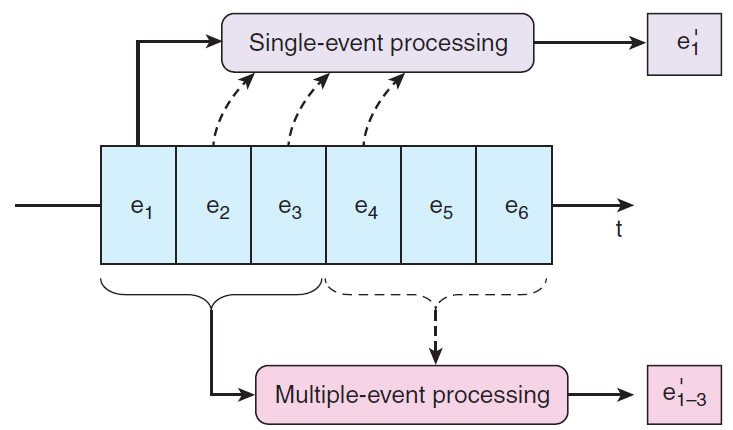
\includegraphics[width=.8\linewidth]{imgs/eventstream_processing.jpg}
% \end{frame}

\framebreak
Amazon Kinesis Data Streams
\i streaming model to ingest data
\i producers send data to a stream that you create and provision by shard
\i each shard provides a maximum of 1 MBps and 1000 data puts per second
\i This data is stored in data records that consist of the following:
\si An incremental sequence number
\si A user-supplied partition key
\ssi load-balance records across shards
\si A data blob
\i By default, records are retained for 24 hours (maximum of 7 days)
\i Data order
\si maintains order through partition key and sequence number
\si producer provides a partition key that determines the shard
\si The shard adds an incremental sequence number to the record
\si Consumers get records by shard, records ordered by sequence number
\si ordering is not guaranteed for requests across shards
\i Operations
\si users must scale shards up and down manually
\si monitor usage with Amazon CloudWatch and modify scale as needed
\si scaling process is called resharding, 
\si split shard into two, or merge two shards
\si avoid shard management by using Kinesis Data Firehose
\ssi automate management to aggregating data into S3/Redshift
% \ssi specify S3 bucket/Redshift cluster, and Kinesis Firehose creates and manages a stream on the user's behalf, depositing the data in specified intervals into the specified location.
\i Kinesis is a regional service, with streams scoped to specific regions
\si all ingested data must travel to the region in which the stream is defined.
\i Costs
\si priced by shard hour, data volume, and data retention period
\si pay for resources you provision (even if not used)
\si Amazon Kinesis Data Firehose is priced by data volume.



\framebreak
Google Pub/Sub
\i messaging service that uses a publisher/subscriber model
\i create a Pub/Sub topic, publish data to that topic
\i applications subscribe to the topic to retrieve ingested data
\i Avoid definition of of shards.
\i push model or pull model
\si push model, the Pub/Sub server sends a request to the subscriber application at a preconfigured URL endpoint
\si pull model, the subscriber application requests messages from the server, and then acknowledges receipt
\i each data (i.e., message) must be base64-encoded and no larger than 10 MB
\si At the time of ingestion, Pub/Sub adds a messageId attribute and a publishTime
\si messageId unique within the topic
\i Data order
\si delivers messages on a best-effort basis, using system-supplied publishTime
\si does not guarantee only-once or in-order delivery: on occasion, a message might be delivered more than once, and out of order
\si subscriber should be idempotent when processing messages and able to handle messages out of order
\si achieve stricter ordering by using application-supplied sequence numbers
\i Pub/Sub does not require provisioning, and handles sharding, replication, and scaling
\si don't need to use partition keys—Pub/Sub manages data partitioning on your behalf
\si less overhead, but fewer guarantees about message ordering.
\i Pub/Sub uses Google's HTTP(S) load balancer to support data ingestion globally across all Google Cloud regions
\si load balancer automatically directs the traffic to Pub/Sub servers in an appropriate region in order to minimize latency.
\i Pub/Sub is priced by data volume
\si does not require resource provisioning, you pay for only the resources you consume

\framebreak
\begin{table}
\centering
\footnotesize
\begin{tabular}{lp{5cm}p{5cm}}
\textbf{Feature} & \textbf{Amazon Kinesis Data Streams} & \textbf{Google Pub/Sub} \\
Unit of deployment & Stream & Topic \\
Unit of provisioning & Shard & N/A (fully managed) \\
Data unit & Record & Message \\
Data source & Producer & Publisher \\
Data destination & Consumer & Subscriber \\
Data partitioning & User-supplied partition key & N/A (fully managed) \\
Retention period & Up to 7 days & Up to 7 days \\
Data delivery order & Service-supplied sequence key (best effort) & Service-supplied publish time (best effort) \\
Max data size & 1 MB  & 10 MB \\
Deployment locality & Regional & Global \\
Pricing model & Per shard-hour, PUT payload units, and optional data retention & Message ingestion and delivery, and optional message retention \\
\end{tabular}%
\end{table}%
\end{frame}

% \begin{frame}[allowframebreaks]{AWS: ingestion}
% \textbf{Batch}

% \i \textbf{AWS DataSync}
% \si move data between on-premises storage and S3/EFS/etc.
% \si on-premises software transfers data via Network File System protocol
% \si pay only for the data you copy

% \i \textbf{AWS Transfer for SFTP} 
% \si transfer files in/out Amazon S3 using Secure File Transfer Protocol




% \framebreak

% \textbf{Stream}

% \i \textbf{Kinesis} 
% \si collect, process, and analyze real-time, streaming data
% \si ingest real-time data such as video, audio, application logs, etc. 
% \si analyze data as it arrives (and not until all data is collected)

% \i \textbf{Kinesis Data Firehose}
% \si load streaming data into storage/analytics
% tools (S3, Elasticsearch, etc.)
% \si automatically scales to match the throughput

% \i \textbf{Kinesis Data Analytics}
% \si analyze streaming data in real time
% \si use SQL to continuously query streaming data
% \si scales automatically to match the volume and throughput rate

% \framebreak

% \i \textbf{Simple Queue Service (Amazon SQS)} 
% \si message queue that decouples microservices/serverless
% \si send/store/receive messages, avoid message loss
% \si \textit{Standard}: max. throughput, best-effort ordering, at-least-once delivery
% \si \textit{FIFO}: exact ordering, exactly-once delivery

% \i \textbf{Simple Notification Service (SNS)}
% \si topics for high-throughput, push-based, many-to-many messaging
% \si fan out messages to a large number of subscriber endpoints
% \end{frame}

{
\bgimg{1}{imgs/awssnowmobile.png}
\begin{frame}{AWS: ingestion}
    
\end{frame}
}





\ssec{Structural patterns for data pipelines}
\begin{frame}{Structural patterns}
Patterns are architectural solutions to problems in software design
\i Address common problems in software development
\si Command pattern
\si Messaging pattern
\si Priority queue pattern
% \si Fan-out pattern
\si Pipes and filters pattern
\end{frame}

\begin{frame}{Command pattern}
encapsulate a request as an object, thereby letting you parameterize clients with different requests, queue or log requests, and support undoable operations” because of the “need to issue requests to objects without knowing anything about the operation being requested or the receiver of the request”

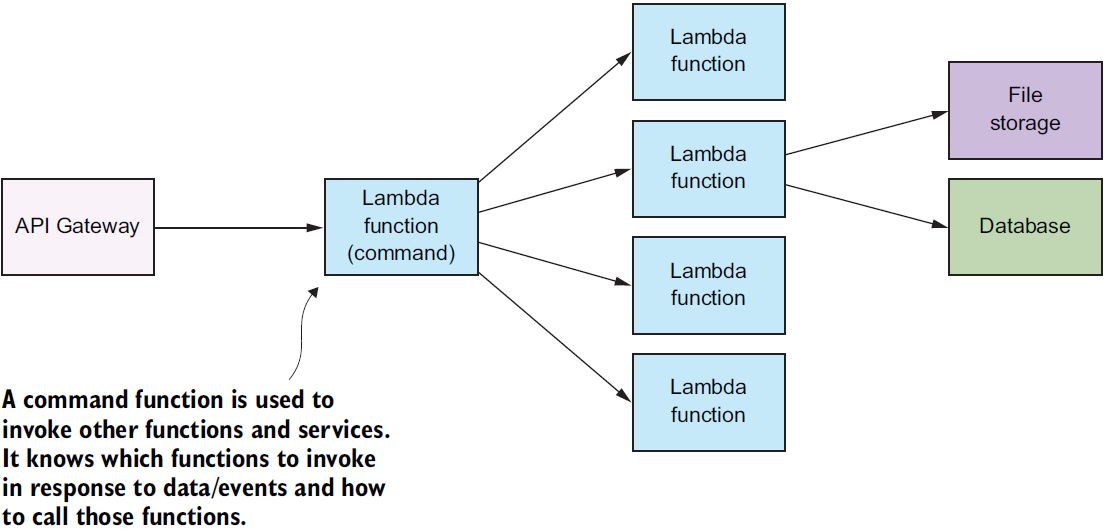
\includegraphics[scale=.4]{imgs/pattern_command.PNG}
\end{frame}

\begin{frame}[allowframebreaks]{Pipes and filters pattern}
Decompose a complex processing task into a sequence of manageable services
\i Components designed to transform data are referred to as filters
\i Connectors that pass data between components are referred to as pipes

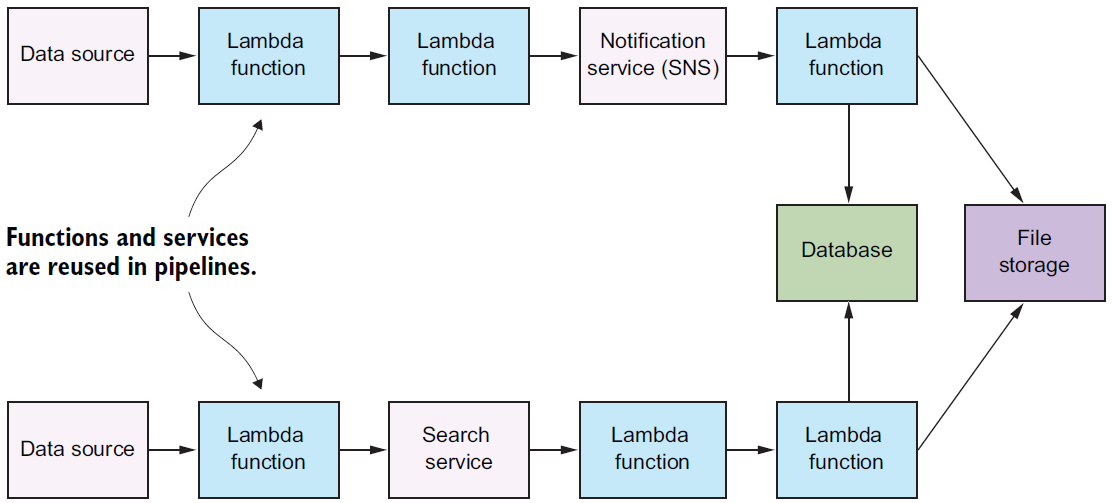
\includegraphics[width=.7\linewidth]{imgs/pattern_pipeline.PNG}
\end{frame}

\begin{frame}{Messaging pattern}
Decoupling functions and services from direct dependence on one another and allowing storage of events/records/requests in a queue. The reliability comes from the fact that if the consuming service goes offline, messages are retained in the queue and can still be processed at a later time.
\i Depending on how the system is designed, a message queue can have a single
sender/receiver or multiple senders/receivers.

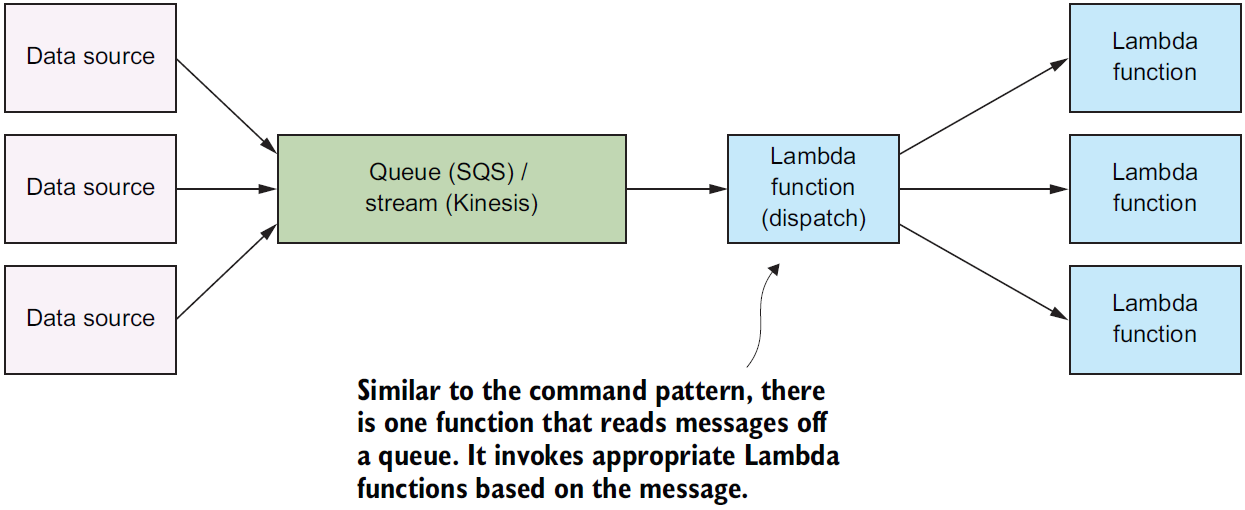
\includegraphics[scale=.4]{imgs/pattern_messaging.PNG}
\end{frame}

\begin{frame}{Priority queue pattern}
Control how and when messages are dealt with
\i Different queues, topics, or streams to feed messages to your functions 
\i High-priority messages go through expensive services with more capacity

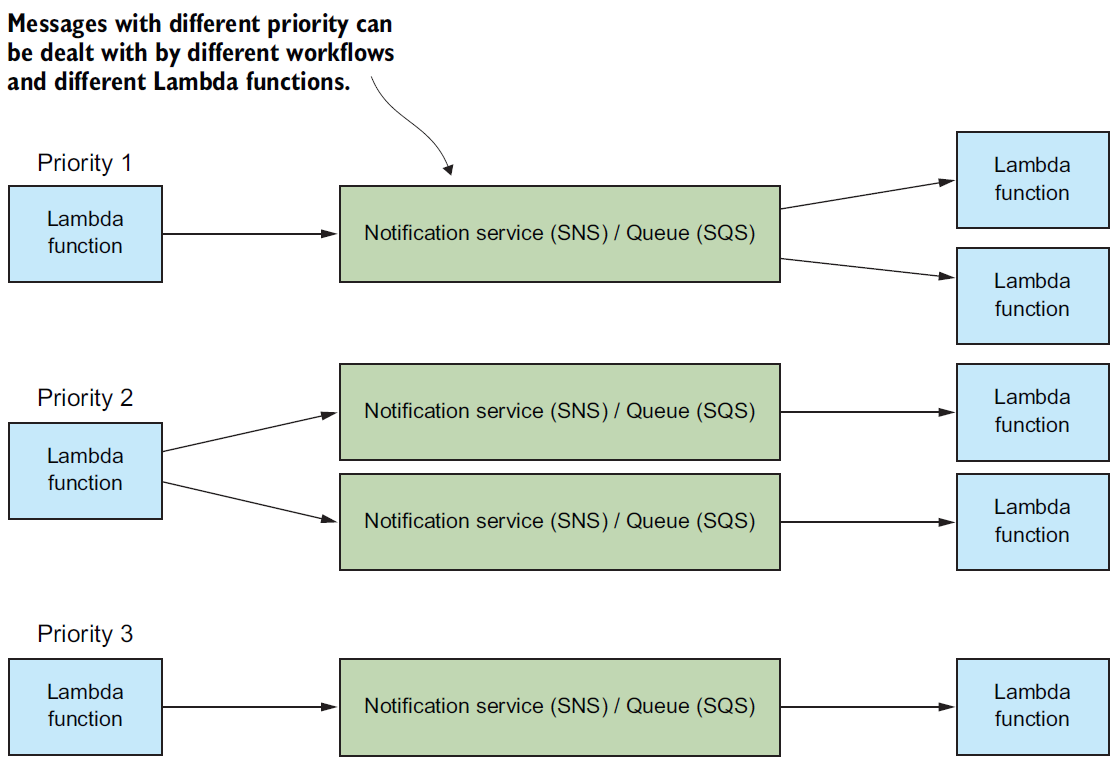
\includegraphics[scale=.4]{imgs/pattern_priority.PNG}
\end{frame}




\sec{Case study}
\ssec{Introduction}

\begin{frame}{Sustainable land management} 
\i Agriculture faces complex challenges to satisfy a population of $9\cdot10^9$ (2050)
\i More water is needed to produce the estimated 60\% of extra food
\i FAO\footnote{\url{http://www.fao.org/water/en/}}: we need a more efficient use of water

\begin{block}{Sustainable land management (United Nations)}
Use of land resources, including soils, water, animals and plants, for the production of goods to meet changing human needs, while simultaneously ensuring the long-term productive potential of these resources and the maintenance of their environmental functions
\end{block}
\end{frame}

\begin{frame}{Scenario}
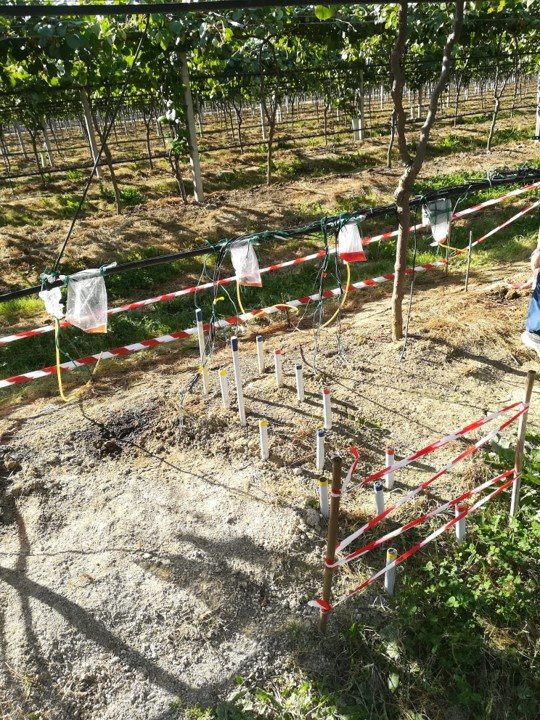
\includegraphics[height=.8\textheight]{imgs/casestudy_real.jpg}
\end{frame}

\begin{frame}{Scenario: water propagation}
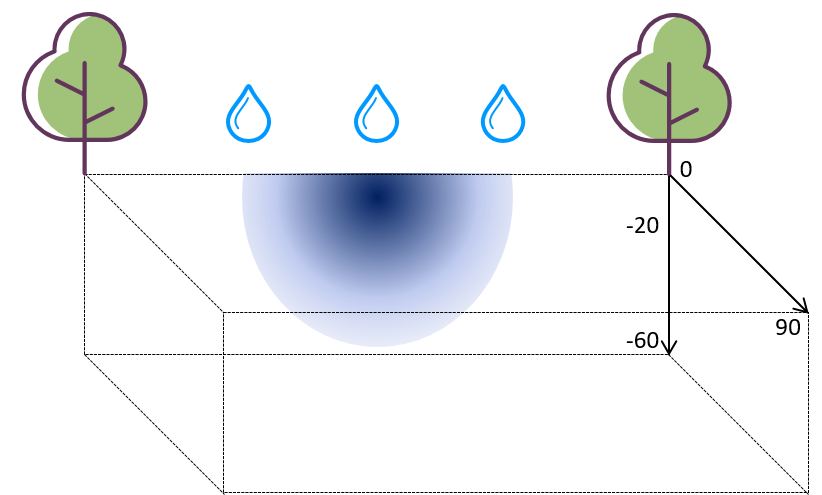
\includegraphics[width=.6\textwidth]{imgs/casestudy.png}
\end{frame}

\begin{frame}{Scenario}
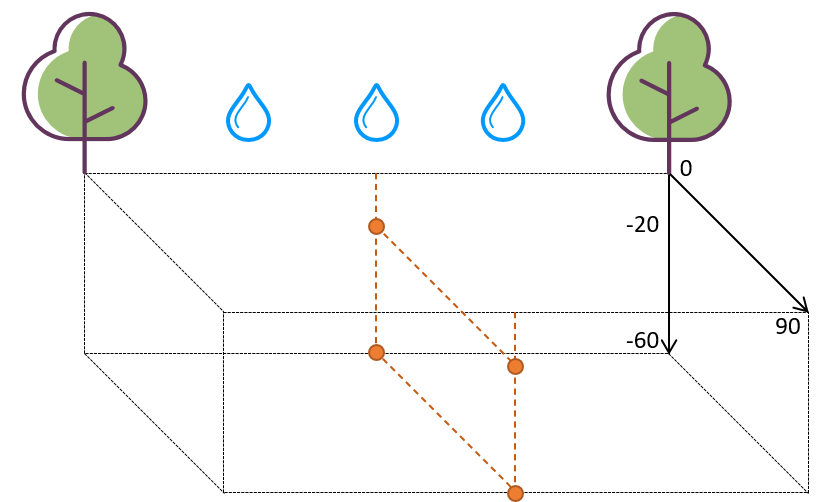
\includegraphics[width=.6\textwidth]{imgs/casestudy_sensors.png}
\end{frame}

\begin{frame}{Smart irrigation: humidity sensors}

\textbf{Goal}: optimization of water resources, provide water only if necessary

\textbf{How}: given humidity sensors displaced on the field, alert the farmer when there is need for irrigation

\textbf{How (technically)}:

\i \textbf{collect} and \textbf{store} raw data from the sources
\i interpolate raw data and \textbf{store} new nata
\i \textbf{alert} when the soil is *too dry*
\i make data available to \textbf{dashboards}
\i ...

\end{frame}

\begin{frame}{Smart-irrigation data pipeline}

\begin{block}{Data pipeline}
Sequences of actions that extract data (or directly analytics and visualization) from various sources
\end{block}

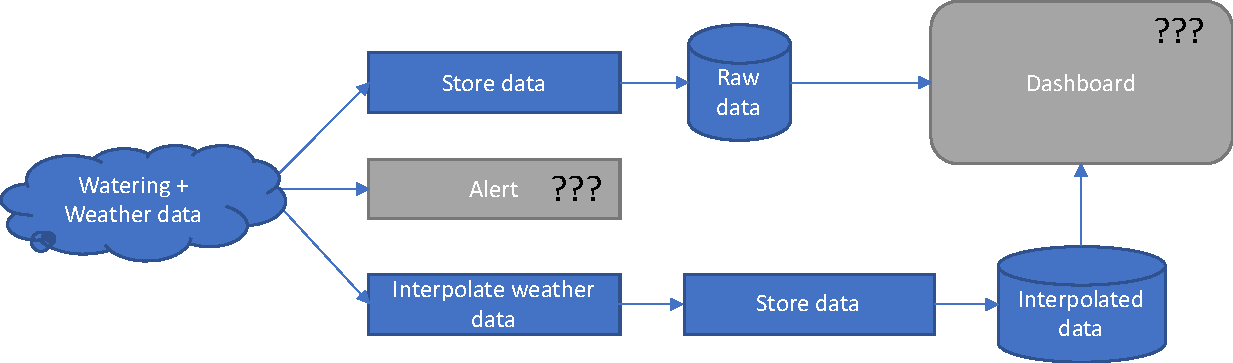
\includegraphics[width=\linewidth]{imgs/pipeline.pdf}
\end{frame}

\begin{frame}{Issues}
\i Building blocks
\i Heterogeneity and compatibility
\end{frame}

\begin{frame}{Issue: building blocks (services)}

\end{frame}
% \ssec{Data pipeline on premises}
% \begin{frame}{Data pipeline on premises}
% 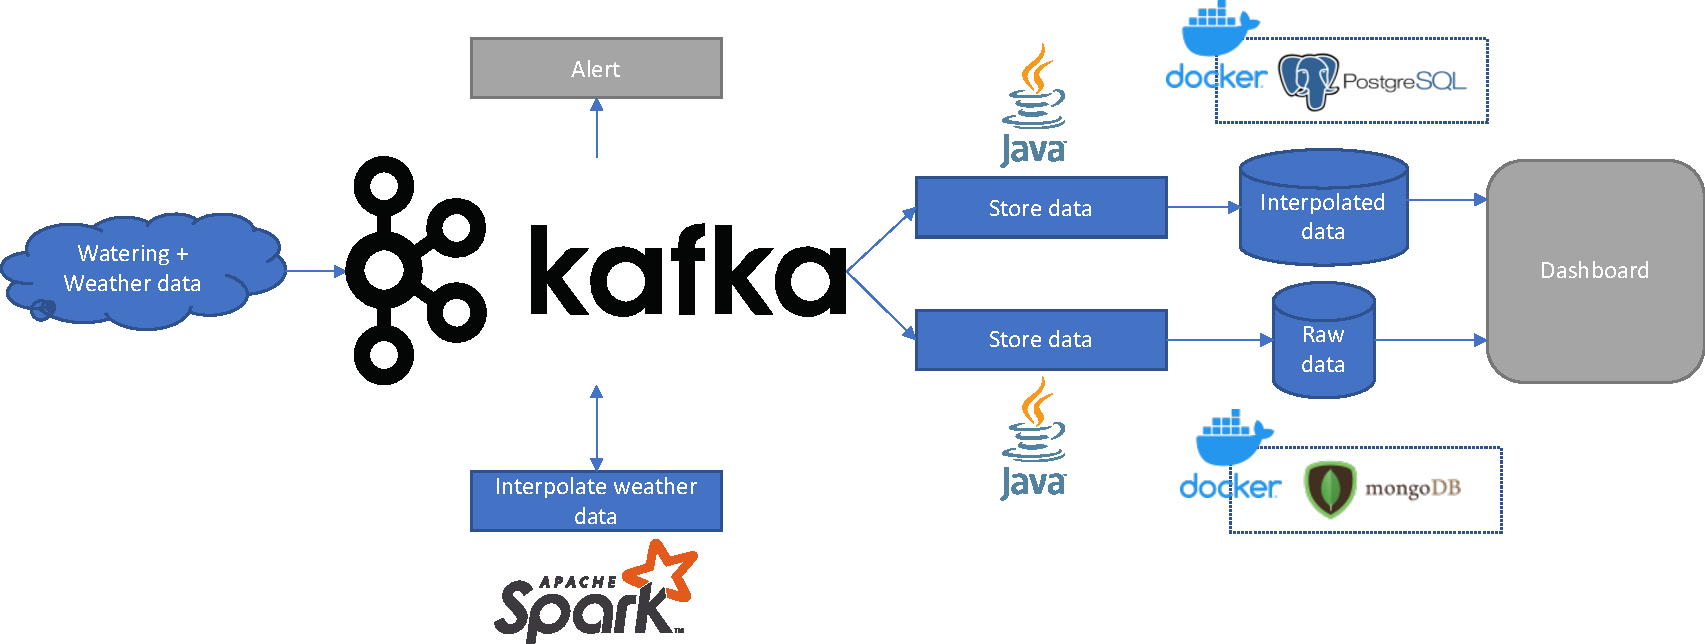
\includegraphics[width=\linewidth]{imgs/pipeline_prem.pdf}
% \end{frame}

\sec{Data pipeline on AWS}

\begin{frame}[allowframebreaks]{AWS}
Useful links and sources
\begin{table}[]
    \centering
    \footnotesize
    \begin{tabular}{ll}
        \textbf{Resource} & \textbf{Link} \\\hline
        AWS Educate & \url{https://aws.amazon.com/it/education/awseducate/}\\
        AWS Console & \url{https://console.aws.amazon.com/console/home?region=us-east-1}\\
        IAM & \url{https://docs.aws.amazon.com/IAM/latest/UserGuide/iam-ug.pdf}\\
        SDK & \url{https://docs.aws.amazon.com/sdk-for-java/latest/developer-guide/home.html}\\
        Lambda & \url{https://docs.aws.amazon.com/lambda/latest/dg/getting-started.html}\\
               & \url{https://console.aws.amazon.com/lambda/home?region=us-east-1\#/functions}\\
        Kinesis & \url{https://docs.aws.amazon.com/streams/latest/dev/introduction.html}\\
        DynamoDB & \url{https://docs.aws.amazon.com/amazondynamodb/latest/developerguide/Introduction.html}\\
    \end{tabular}
\end{table}

Amazon Web Services (AWS) is a platform of web services
\i computing, storing, and networking, at different abstraction layers 
\i web service means services controlled via a (visual) web interface
\i EC2, which offers virtual servers, and S3, which offers storage capacity
\si E.g., Linux server with an optimized distribution
called Amazon Linux
\si Virtual servers can fail, so you need at least two of them
\si The load balancer will distribute the traffic between them
    
Clouds are often divided into types
\i Public, public usage
\i Private, private usage
\i Hybrid, a mixture of a public and a private cloud
AWS is a public cloud

Cloud computing services also have several classifications:
\i Infrastructure as a service (IaaS)
\si fundamental resources like computing,
storage, and networking
\i Platform as a service (PaaS)
\si deploy applications to
cloud platforms (AWS Elastic Beanstalk, Heroku)
\i Software as a service (SaaS)
\si provide software running in
the cloud (Amazon WorkSpaces, and Microsoft Office 365)

AWS product portfolio contains IaaS, PaaS, and SaaS
\end{frame}

\begin{frame}[allowframebreaks]{Accessing the cloud}
Most cloud services can be accessed in multiple ways. First, most
support access via the web, thus permitting intuitive point and click
access without any programming or even local software installation
(beyond a web browser) on your part. The availability of such
intuitive interfaces is part of the attraction of cloud services.

A web interface becomes tedious if the same or similar actions
must be performed repeatedly. In such cases, you likely want to
write programs that issue requests to cloud services on your behalf.
Fortunately, most cloud services support such programmatic access.
Typically, they support a Representational State Transfer (REST)
application programming interface (API) that permits requests to be
transmitted via the secure Hypertext Transfer Protocol (HTTPS) that
is used by web browsers. (This common use of HTTPS is not a
coincidence: the web interfaces discussed in the first paragraph are
often implemented via browser-hosted Javascript programs that
generate such REST messages.) REST APIs are the key to
programmatic interactions with cloud services.

One way to interact with cloud services programmatically is to
write programs that generate REST messages directly. However,
while constructing REST messages “by hand” may appeal to hardcore
system programmers, you will normally want to access cloud
services via software development kits (SDKs) that you install on
your computer. Such SDKs permit access from programming
languages such as Python (our choice in this book), C++, Go, Java,
PHP, and Ruby.
\end{frame}


\begin{frame}{Interacting with AWS}

\i Management Console (web-based) 
\i Command-line interface
\i SDK, call AWS from within your application
\i Blueprints, a system description containing all services and dependencies
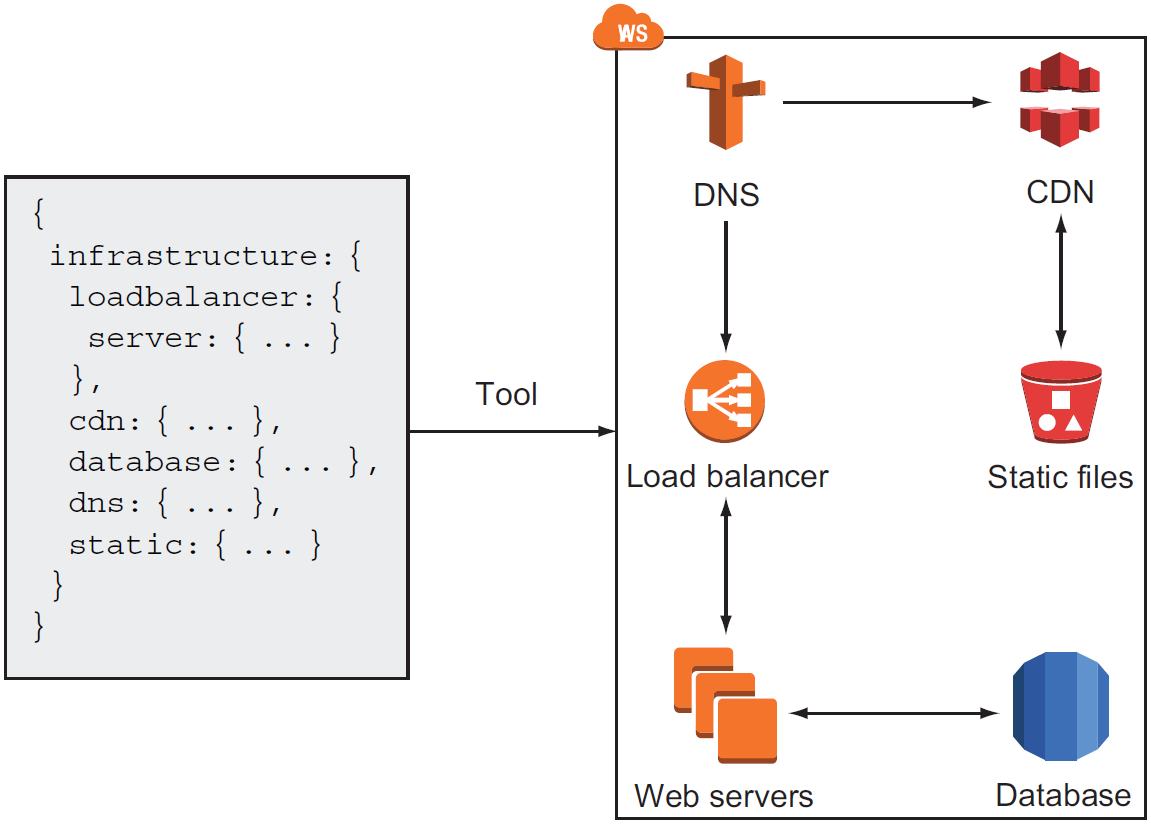
\includegraphics[width=\textwidth]{imgs/aws_blueprint.PNG}
\end{frame}

\begin{frame}{Creating an infrastructure}
    Infrastructure as code
Infrastructure as code describes the idea of using a high-level programming language to
control IT systems. In software development tools like automated tests, code repositories,
and build servers are increasing the quality of software engineering. If your infrastructure
can be treated as code, you can apply the same techniques to infrastructure
code that you do to your application code. In the end, you’ll improve the quality of
your infrastructure by using automated tests, code repositories, and build servers.
WARNING Don’t mix up the terms infrastructure as code and infrastructure as a
service (IaaS)! IaaS means renting servers, storage, and network with a pay-peruse
pricing model.

If you want to use cloud advantages like scaling the number of servers depending on
the current load or building a highly available infrastructure, you’ll need to start new
virtual servers several times a day. On top of that, the number of virtual servers you’ll
have to supply with updates will grow. The steps required to deploy an application
don’t change, but as figure 5.1 shows, you need to perform them on multiple servers.
Deploying software manually to a growing number of servers becomes impossible over
time and has a high risk of human failure. This is why we recommend that you automate
the deployment of applications.

A simple but powerful and flexible way of automating application deployment is to
run a script on server startup. To go from a plain OS to a fully installed and configured
server, you need to follow these three steps:
1 Start a plain virtual server containing just an OS.
2 Execute a script at the end of the boot process.
3 Install and configure your applications with the help of a script.
\end{frame}

\begin{frame}{Service categorization}
Main service categories
\i Compute services, computing power and memory (e.g., virtual servers)
\i App services, solutions for common use cases (message queues, topics, and searching)
\i Deployment and administration, grant/revoke access, monitor servers, deploy applications.
\i Storage, collect and persist data
\i Networking, define private networks, DNS, etc.
\end{frame}

\begin{frame}{Cloud providers}
    Comparing alternatives
AWS isn’t the only cloud computing provider. Microsoft and Google have cloud offerings
as well.
OpenStack is different because it’s open source and developed by more than 200
companies including IBM, HP, and Rackspace. Each of these companies uses Open-
Stack to operate its own cloud offerings, sometimes with closed source add-ons. You
could run your own cloud based on OpenStack, but you would lose most of the benefits
outlined in section 1.3.
Comparing cloud providers isn’t easy, because open standards are mostly missing.
Functionality like virtual networks and message queuing are realized differently. If you
know what features you need, you can compare the details and make your decision.
\end{frame}

\begin{frame}{Data pipeline on AWS cloud}
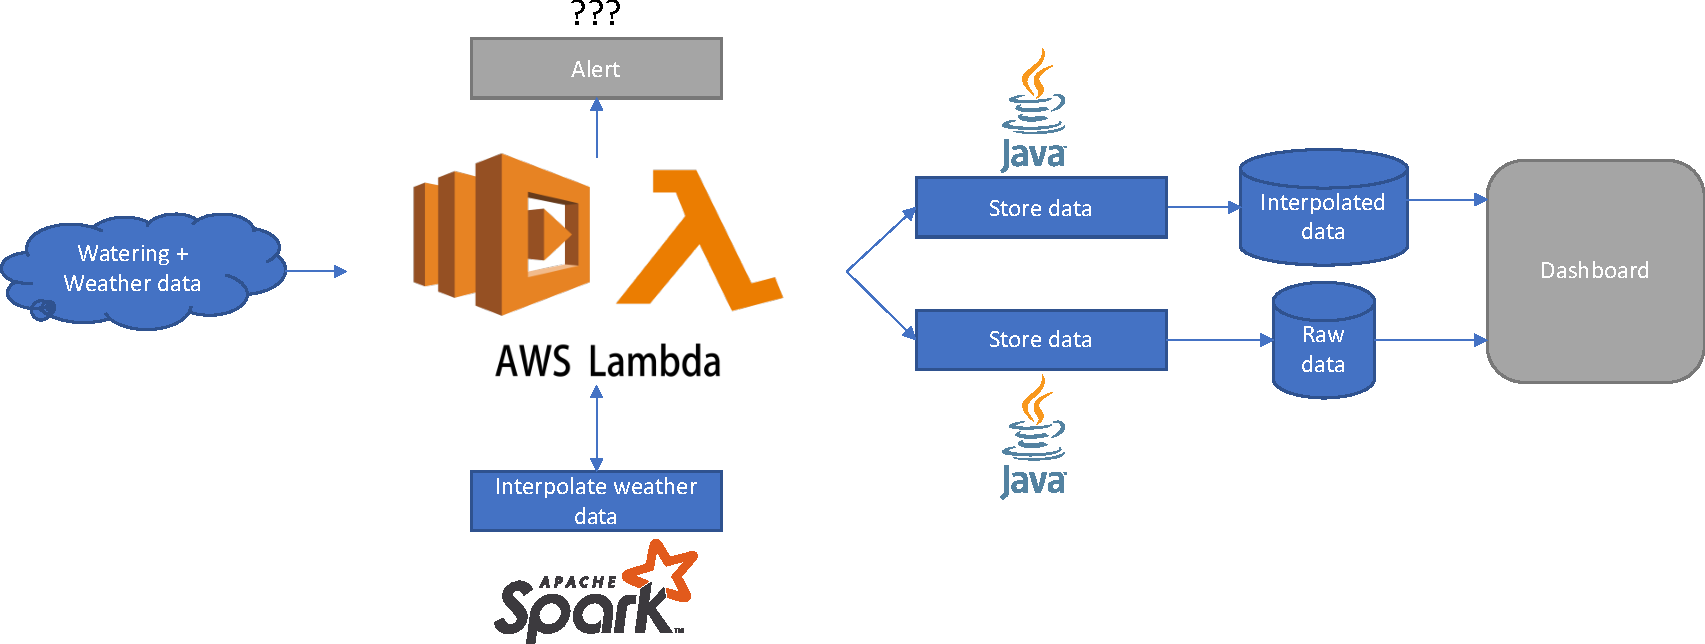
\includegraphics[width=\linewidth]{imgs/pipeline_aws.pdf}
\end{frame}

\ssec{Authentication and authorization}
\begin{frame}[fragile,allowframebreaks]{AWS - Identity and Access Management}

\textbf{Identity and Access Management (IAM)}
\i web service that controls access to AWS resources
\i IAM controls who is \textit{authenticated} and \textit{authorized} to use resources

\textbf{User}
\i unique identity recognized by AWS services and applications
\si individual, system, or application accessing AWS services
\i similar to user in an operating system like Windows or UNIX

After the account creation
\i begin with a single sign-in identity that has complete access
to all AWS services and resources in the account
\i i.e., a \lstinline{root user}
\i do not use the root user for your everyday tasks, even the administrative ones
\i use the root user only to create your first IAM user
\i specify permissions to control which operations a user can perform

What can a user do?
\i place requests to web services such as Amazon S3 and Amazon EC2
\i If permitted, a user has access to all of the resources under the AWS account
\i sers can make requests to AWS services using security credentials
\i \textbf{Explicit} permissions govern a user's ability to call AWS services

\textbf{IAM role}
\i set of permissions for making AWS service requests
\i trusted entities (e.g., such as IAM users) assume roles
\si \textbf{not} associated with a specific user or group
\i delegate access with defined permissions to trusted entities without having to share long-term access keys
\i there is no limit to the number of IAM roles you can assume

Role vs user
\i user has permanent long-term credentials and is used to directly interact with AWS services
\i role does not have any credentials and cannot make direct requests to AWS services
\i IAM roles are meant to be assumed by authorized entities, such as IAM users, applications, or an AWS service such as EC2.

\textbf{Policy}
\i an object in AWS that, when associated with an identity or resource, defines their permissions
\i AWS evaluates these policies when an IAM principal (user or role) makes a request
\i Permissions in the policies determine whether the request is allowed or denied
\i You manage access in AWS by creating policies and attaching them to IAM identities (users, groups of users, or roles)
\i six types of policies (listed in order of frequency)
\si Identity-based policies, grant permissions to an identity.
\si Resource-based policies, e.g. resource-based policies are Amazon S3 bucket policies
\si Permissions boundaries, maximum permissions that the identity-based policies can grant to an entity
\si Service control policy (SCP), maximum permissions for members of an organization or organizational unit (OU)
\si Access control lists (ACLs), which accounts can access the resource to which the ACL is attached.
\si Session policies, limit the permissions that the role or user's identity-based policies grant to the session
\end{frame}

\begin{frame}[fragile,allowframebreaks]{AWS CLI and authentication}
We will mainly refer to the CLI interface
\begin{lstlisting}
Synopsis
********
   aws [options] <command> <subcommand> [parameters]

Description
***********
A unified tool to manage your AWS services.
\end{lstlisting}

First of all it is necessary to install the CLI (version 2)
\i See {\footnotesize \url{https://docs.aws.amazon.com/cli/latest/userguide/install-cliv2.html}}

\framebreak
This is your AWS account

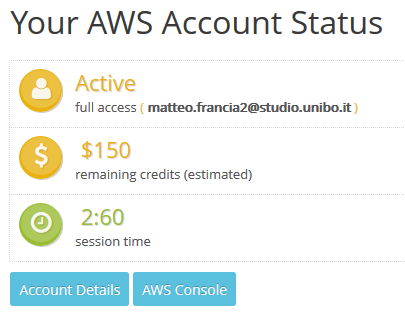
\includegraphics[scale=.5]{imgs/aws_account.PNG}

\framebreak
Click on ``Account Details'' to get your secrets

\i Copy the content into the file \lstinline{~/.aws/configure}
\i \textbf{All examples assume that you have setup your credentials in the credentials file}
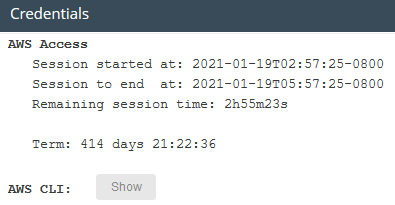
\includegraphics[scale=.5]{imgs/aws_account1.PNG}

\framebreak
Run \lstinline{aws configure}
\i Confirm \lstinline{AWS Access Key ID}
\i Confirm \lstinline{AWS Secret Access Key}
\i Set \lstinline{Default region name} to \lstinline{us-east-1}
\i Set \lstinline{Default output format} to \lstinline{json} 

It is also possible to configure an AWS profile
\i A (named) profile is a collection of settings and credentials
\i If profile is specified, its settings and credentials are used to run a command
\i When no profile is explicitly referenced, use ``default'' 
\si \textbf{We stick to ``default''}

\end{frame}

\ssec{NoSQL}
\begin{frame}[fragile,allowframebreaks]{AWS - NoSQL with DynamoDB}

The following are the basic DynamoDB components:

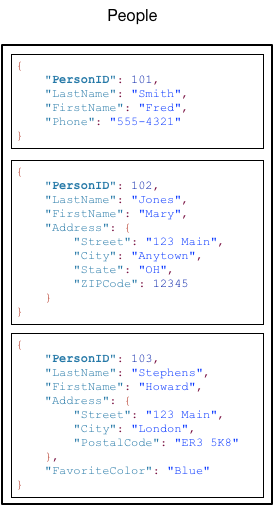
\includegraphics[height=\textheight]{imgs/HowItWorksPeople.png}

\textbf{Tables}
\i a collection of (data) items
\i e.g., example table called People

\textbf{Items}
\i a group of attributes that is uniquely identifiable among all others
\i Each table contains zero or more items
\si no limit to the number of items you can store in a table.
\i Items tuples in other database systems
\si In the People table, each item represents a person. 
\i Each item in the table has a unique identifier, or primary key
\si In the People table, the primary key consists of one attribute (PersonID)

\textbf{Attributes} 
\i a fundamental data element that is not broken down any further
\i e.g., an item in the People table contains attributes PersonID, LastName, FirstName
\i Most of the attributes are scalar (have only one value)
\si Strings and numbers are common examples of scalars
\i Some of the items have a nested attribute (Address)
\si up to 32 levels deep

\textbf{Schemaless}
\i Other than the primary key, the People table is schemaless
\i neither the attributes nor their data types need to be defined beforehand
\i Each item can have its own distinct attributes.

\textbf{Primary Key}
\i To create a table, you must specify the primary key of the table
\i The primary key uniquely identifies each item in the table, 
\si no two items can have the same key.

Two types of primary keys
\i Partition key: a simple primary key, composed of one attribute known as the partition key
\si key values as inputs to an internal hash function
\si The hash function determines the partition (physical storage internal to DynamoDB) in which the item will be stored
\si access any item in the People table directly by providing the PersonId

\i composite primary key: Partition key and sort key (two attributes)
\si first attribute is the partition key
\si second attribute is the sort key
\si items in same partition key value are stored together, in sorted order by sort key

\textbf{Secondary Indexes}
\i one or more secondary indexes per table
\i query data using an alternate key (additionally to queries against primary key) 
\i indexes are automatically maintained on add, update, or delete

Two types of indexes
\i \textbf{Global secondary} has partition and sort keys different from those on table
\i \textbf{Local secondary} has the same partition key but a different sort key
\i Each table has a quota of 20 global and 5 local indexes

How do we shape the schema?
\i \url{https://cloud.google.com/bigtable/docs/schema-design}

\begin{lstlisting}
$ aws dynamodb create-table \
    --table-name soil-humidity \
    --attribute-definitions AttributeName=field,AttributeType=S AttributeName=timestamp,AttributeType=S \
    --key-schema AttributeName=field,KeyType=HASH AttributeName=timestamp,KeyType=RANGE \
    --provisioned-throughput ReadCapacityUnits=1,WriteCapacityUnits=1
    
$ aws dynamodb create-table \
    --table-name interpolate-soil-humidity \
    --attribute-definitions AttributeName=field,AttributeType=S AttributeName=timestamp,AttributeType=S \
    --key-schema AttributeName=field,KeyType=HASH AttributeName=timestamp,KeyType=RANGE \
    --provisioned-throughput ReadCapacityUnits=1,WriteCapacityUnits=1
\end{lstlisting}

Amazon DynamoDB is available in multiple AWS Regions around the world. Each Region is independent and isolated from other AWS Regions. For example, if you have a table called People in the us-east-2 Region and another table named People in the us-west-2 Region, these are considered two entirely separate tables. For a list of all the AWS Regions in which DynamoDB is available, see AWS Regions and Endpoints in the Amazon Web Services General Reference.

Every AWS Region consists of multiple distinct locations called Availability Zones. Each Availability Zone is isolated from failures in other Availability Zones, and provides inexpensive, low-latency network connectivity to other Availability Zones in the same Region. This allows rapid replication of your data among multiple Availability Zones in a Region.

When your application writes data to a DynamoDB table and receives an HTTP 200 response (OK), the write has occurred and is durable. The data is eventually consistent across all storage locations, usually within one second or less.

DynamoDB supports eventually consistent and strongly consistent reads.

Eventually Consistent Reads

When you read data from a DynamoDB table, the response might not reflect the results of a recently completed write operation. The response might include some stale data. If you repeat your read request after a short time, the response should return the latest data.

Strongly Consistent Reads

When you request a strongly consistent read, DynamoDB returns a response with the most up-to-date data, reflecting the updates from all prior write operations that were successful. However, this consistency comes with some disadvantages:

    A strongly consistent read might not be available if there is a network delay or outage. In this case, DynamoDB may return a server error (HTTP 500).

    Strongly consistent reads may have higher latency than eventually consistent reads.

    Strongly consistent reads are not supported on global secondary indexes.

    Strongly consistent reads use more throughput capacity than eventually consistent reads. For details, see Read/Write Capacity Mode

Note

DynamoDB uses eventually consistent reads, unless you specify otherwise. Read operations (such as GetItem, Query, and Scan) provide a ConsistentRead parameter. If you set this parameter to true, DynamoDB uses strongly consistent reads during the operation.


If you choose provisioned mode, you specify the number of reads and writes per second that you require for your application. You can use auto scaling to adjust your table’s provisioned capacity automatically in response to traffic changes. This helps you govern your DynamoDB use to stay at or below a defined request rate in order to obtain cost predictability.

Provisioned mode is a good option if any of the following are true:

    You have predictable application traffic.

    You run applications whose traffic is consistent or ramps gradually.

    You can forecast capacity requirements to control costs.



Read Capacity Units and Write Capacity Units

For provisioned mode tables, you specify throughput capacity in terms of read capacity units (RCUs) and write capacity units (WCUs):

    One read capacity unit represents one strongly consistent read per second, or two eventually consistent reads per second, for an item up to 4 KB in size. Transactional read requests require two read capacity units to perform one read per second for items up to 4 KB. If you need to read an item that is larger than 4 KB, DynamoDB must consume additional read capacity units. The total number of read capacity units required depends on the item size, and whether you want an eventually consistent or strongly consistent read. For example, if your item size is 8 KB, you require 2 read capacity units to sustain one strongly consistent read per second, 1 read capacity unit if you choose eventually consistent reads, or 4 read capacity units for a transactional read request. For more information, see Capacity Unit Consumption for Reads.

Note

To learn more about DynamoDB read consistency models, see Read Consistency.

One write capacity unit represents one write per second for an item up to 1 KB in size. If you need to write an item that is larger than 1 KB, DynamoDB must consume additional write capacity units. Transactional write requests require 2 write capacity units to perform one write per second for items up to 1 KB. The total number of write capacity units required depends on the item size. For example, if your item size is 2 KB, you require 2 write capacity units to sustain one write request per second or 4 write capacity units for a transactional write request. For more information, see Capacity Unit Consumption for Writes.



Putting data

\begin{lstlisting}
$ aws dynamodb create-table \
    --table-name soil-humidity \
    --attribute-definitions AttributeName=field,AttributeType=S AttributeName=timestamp,AttributeType=S \
    --key-schema AttributeName=field,KeyType=HASH AttributeName=timestamp,KeyType=RANGE \
    --provisioned-throughput ReadCapacityUnits=1,WriteCapacityUnits=1

$ aws dynamodb create-table \
    --table-name interpolate-soil-humidity \
    --attribute-definitions AttributeName=field,AttributeType=S AttributeName=timestamp,AttributeType=S \
    --key-schema AttributeName=field,KeyType=HASH AttributeName=timestamp,KeyType=RANGE \
    --provisioned-throughput ReadCapacityUnits=1,WriteCapacityUnits=1

$ aws dynamodb delete-table --table-name soil-humidity

$ aws dynamodb delete-table --table-name interpolate-soil-humidity

$ aws dynamodb list-tables

$ aws dynamodb put-item \
    --table-name soil-humidity \
    --item \
    '{"field": {"S": "field-01"}, "timestamp": {"S": "1611226870"}, "xx": {"N": "0"}, "yy": {"N": "-20"}, "value": {"N": "-17"}}'

$ aws dynamodb put-item \
    --table-name soil-humidity \
    --item \
    '{"field": {"S": "field-01"}, "timestamp": {"N": "1611226880"}, "xx": {"S": "0"}, "yy": {"S": "-20"}, "value": {"S": "-20"}}'
    
$ aws kinesis put-record --stream-name events --partition-key soilhumidity --cli-binary-format raw-in-base64-out --data \
    '{"field": "field-01", "timestamp": "1611226890", "xx": "0", "yy": "-20", "value": "-23", "message": "Hello from AWS CLI!"}'

$ aws kinesis put-record --stream-name events --partition-key soilhumidity --cli-binary-format raw-in-base64-out --data \
    '{"field": "field-01", "timestamp": "1611226900", "xx": "0", "yy": "-20", "value": "-26", "message": "Hello from AWS CLI!"}'
\end{lstlisting}



The Query operation in Amazon DynamoDB finds items based on primary key values.

You must provide the name of the partition key attribute and a single value for that attribute. Query returns all items with that partition key value. Optionally, you can provide a sort key attribute and use a comparison operator to refine the search results. 

To specify the search criteria, you use a key condition expression—a string that determines the items to be read from the table or index.

You must specify the partition key name and value as an equality condition.

You can optionally provide a second condition for the sort key (if present). The sort key condition must use one of the following comparison operators:

    a = b — true if the attribute a is equal to the value b

    a < b — true if a is less than b

    a <= b — true if a is less than or equal to b

    a > b — true if a is greater than b

    a >= b — true if a is greater than or equal to b

    a BETWEEN b AND c — true if a is greater than or equal to b, and less than or equal to c.

The following function is also supported:

    begins_with (a, substr)— true if the value of attribute a begins with a particular substring.



\begin{lstlisting}
$ aws dynamodb query \
    --table-name soil-humidity \
    --key-condition-expression "field = :n" \
    --expression-attribute-values '{":n":{"S":"field-01"}}'

$ aws dynamodb query \
    --table-name soil-humidity \
    --key-condition-expression "field = :n" \
    --expression-attribute-values '{":n":{"S":"field-02"}}'
    
aws dynamodb delete-table --table-name soil-humidity

aws dynamodb delete-table --table-name interpolate-soil-humidity

aws dynamodb create-table \
  --table-name soil-humidity \
  --attribute-definitions AttributeName=field,AttributeType=S AttributeName=timestamp,AttributeType=S \
  --key-schema AttributeName=field,KeyType=HASH AttributeName=timestamp,KeyType=RANGE \
  --provisioned-throughput ReadCapacityUnits=1,WriteCapacityUnits=1

aws dynamodb create-table \
  --table-name interpolate-soil-humidity \
  --attribute-definitions AttributeName=field,AttributeType=S AttributeName=sensorid,AttributeType=S \
  --key-schema AttributeName=field,KeyType=HASH AttributeName=sensorid,KeyType=RANGE \
  --provisioned-throughput ReadCapacityUnits=1,WriteCapacityUnits=1

aws dynamodb query \
  --table-name soil-humidity \
  --key-condition-expression "field = :n" \
  --expression-attribute-values '{":n":{"S":"field-01"}}'

aws dynamodb query \
  --table-name soil-humidity \
  --key-condition-expression "field = :n" \
  --expression-attribute-values '{":n":{"S":"field-02"}}'

aws dynamodb query \
  --table-name soil-humidity \
  --key-condition-expression "field = :n" \
  --expression-attribute-values '{":n":{"S":"field-00"}}'

aws dynamodb query \
  --table-name interpolate-soil-humidity \
  --key-condition-expression "field = :n" \
  --expression-attribute-values '{":n":{"S":"field-00"}}'
\end{lstlisting}

Filter Expressions for Query

If you need to further refine the Query results, you can optionally provide a filter expression. A filter expression determines which items within the Query results should be returned to you. All of the other results are discarded.

A filter expression is applied after a Query finishes, but before the results are returned. Therefore, a Query consumes the same amount of read capacity, regardless of whether a filter expression is present.

A Query operation can retrieve a maximum of 1 MB of data. This limit applies before the filter expression is evaluated.

A filter expression cannot contain partition key or sort key attributes. You need to specify those attributes in the key condition expression, not the filter expression.

The syntax for a filter expression is identical to that of a condition expression. Filter expressions can use the same comparators, functions, and logical operators as a condition expression, with the addition of the not-equals operator (<>). For more information, see Condition Expressions.

Example

The following AWS CLI example queries the Thread table for a particular ForumName (partition key) and Subject (sort key). Of the items that are found, only the most popular discussion threads are returned—in other words, only those threads with more than a certain number of Views. 

\begin{lstlisting}

$ aws dynamodb query \
    --table-name Thread \
    --key-condition-expression "ForumName = :fn and Subject = :sub" \
    --filter-expression "#v >= :num" \
    --expression-attribute-names '{"#v": "Views"}' \
    --expression-attribute-values file://values.json
 
\end{lstlisting}
The arguments for --expression-attribute-values are stored in the values.json file. 
\begin{lstlisting}
{
    ":fn":{"S":"Amazon DynamoDB"},
    ":sub":{"S":"DynamoDB Thread 1"},
    ":num":{"N":"3"}
}
\end{lstlisting}

\end{frame}

\ssec{Event streams}
\begin{frame}[fragile,allowframebreaks]{AWS - Event streams with Kinesis}
Creating a Kinesis stream

Kinesis Data Stream
\i A Kinesis data stream is a set of shards. 
\i Each shard has a sequence of data records. 
\i Each data record has a sequence number that is assigned by Kinesis Data Streams.

Data Record
\i unit of data stored in a Kinesis data stream. 
\i Data records are composed of a sequence number, a partition key, and a data blob
\i Kinesis Data Streams does not inspect, interpret, or change the data in the blob in any way. 
\i A data blob can be up to 1 MB.

Retention Period
\i the length of time that data records are accessible after they are added to the stream
\i A stream’s retention period is set to a default of 24 hours after creation.
\i Additional charges apply for streams with a retention period set to more than 24 hours. For more information, see Amazon Kinesis Data Streams Pricing

Producer
\i Producers put records into Amazon Kinesis Data Streams

Consumer
\i Get and process records from Amazon Kinesis Data Streams
\i Also known as Amazon Kinesis Data Streams Application

Two types of consumers that you can develop
\i shared fan-out consumers 
\i enhanced fan-out consumers
\i The output of a Kinesis Data Streams application can be input for another stream, enabling you to create complex topologies that process data in real time. 
\i An application can also send data to a variety of other AWS services. 
\i There can be multiple applications for one stream, and each application can consume data from the stream independently and concurrently.

Shard
\i sequence of data records in a stream
\i A stream is composed of one or more shards, each of which provides a fixed unit of capacity. 
\i Each shard can support up to 5 transactions per second for reads, up to a maximum total data read rate of 2 MB per second and up to 1,000 records per second for writes, up to a maximum total data write rate of 1 MB per second (including partition keys). The data capacity of your stream is a function of the number of shards that you specify for the stream. The total capacity of the stream is the sum of the capacities of its shards.

If your data rate increases, you can increase or decrease the number of shards allocated to your stream. For more information, see Resharding a Stream.


Partition Key
\i A partition key is used to group data by shard within a stream. Kinesis Data Streams segregates the data records belonging to a stream into multiple shards. It uses the partition key that is associated with each data record to determine which shard a given data record belongs to. Partition keys are Unicode strings, with a maximum length limit of 256 characters for each key. An MD5 hash function is used to map partition keys to 128-bit integer values and to map associated data records to shards using the hash key ranges of the shards. When an application puts data into a stream, it must specify a partition key. 

\begin{lstlisting}
$ aws kinesis create-stream --stream-name events --shard-count 2

$ aws kinesis delete-stream --stream-name events

$ aws kinesis describe-stream --stream-name events

$ aws kinesis get-shard-iterator --stream-name=events \
    --shard-id=shardId-000000000000 --shard-iterator-type=TRIM_HORIZON
{
    "ShardIterator": "iterator-id-00"
}

$ aws kinesis get-records --shard-iterator "iterator-id-00"
{
    "Records": [],
    "NextShardIterator": "iterator-id-01",
    "MillisBehindLatest": 0
}

$ aws kinesis get-records --shard-iterator  "iterator-id-01"
{
    "Records": [],
    "NextShardIterator": "iterator-id-02",
    "MillisBehindLatest": 0
}
\end{lstlisting}

Created a stream with two shards
\i events sent will be written to one or either of the two shards
\i stream processing apps read events from all shards
\i Status {\footnotesize\url{https://console.aws.amazon.com/kinesis/home?region=us-east-1#/streams/list}}

We specified that the shard iterator should be of type TRIM\_HORIZON. This is AWS jargon
for the oldest events in the shard that have not yet been trimmed—expired for
being too old. At the time of writing, records are trimmed from a Kinesis stream after
a fixed period of 24 hours

\framebreak

Creating the producer using Amazon SDK
\i need to be able to send events to it from all our various client applications
\si E.g., Producer in Python using Amazon SDK (boto3)
\end{frame}

\ssec{Serverless}
\begin{frame}{Going serverless}
Amazon AWS Lambda as a case study
\i Execute code in a massively parallelized way in response to events
\i Elastic Compute Cloud (EC2) servers run the code
\si E.g., Linux server with distribution
Amazon Linux
\i See also Microsoft Azure Functions, IBM Bluemix, Google Cloud Functions

AWS lambda
\i The Lambda runtime invokes a lambda function multiple times in parallel
\i Invocation supports push/pull event models
\i \textbf{Lambda function}: code + configuration + dependencies
\i Compute service that executes code written in JavaScript/Python/C\#/Java
\i Source code (JARs or DLLs) is zipped up and deployed to a container

In AWS, every Lambda function is a granular service
\i Inputs and outputs should be clearly defined (i.e., a clear interface)
\si Similar to the compute-as-glue architecture we described previously
\i Make sure your function follows the single-responsibility principle
\i Make the function idempotent (i.e., given an input produce the same output)
\i Clearly define an interface for the function
\si Make sure inputs and outputs are clearly stated
\i Function are black-boxes
\si consumer should not have to know how it works

\end{frame}

\begin{frame}[fragile,allowframebreaks]{AWS - Serverless with Lambda}
AWS Lambda is a compute service that lets you run code without provisioning or managing servers.
Lambda runs your code only when needed and scales automatically, from a few requests per day
to thousands per second. You pay only for the compute time that you consume—there is no charge
when your code is not running. With Lambda, you can run code for virtually any type of application or
backend service, all with zero administration. Lambda runs your code on a high-availability compute
infrastructure and performs all of the administration of the compute resources, including server and
operating system maintenance, capacity provisioning and automatic scaling, code monitoring and
logging.

When using Lambda, you are responsible only for your code. Lambda manages the compute fleet that
offers a balance of memory, CPU, network, and other resources. This is in exchange for flexibility, which
means you cannot log in to compute instances, or customize the operating system on provided runtimes.
These constraints enable Lambda to perform operational and administrative activities on your behalf,
including provisioning capacity, monitoring fleet health, applying security patches, deploying your code,
and monitoring and logging your Lambda functions.

Create a function
\i \url{https://console.aws.amazon.com/lambda/home?region=us-east-1#/functions}

The following "create-function" example creates a Lambda function
named "my-function".
\begin{lstlisting}
$ aws iam create-role --role-name lambda-execute

$ aws iam attach-role-policy \
    --policy-arn arn:aws:iam::aws:policy/service-role/AWSLambdaKinesisExecutionRole --role-name lambda-execute

$ aws iam attach-role-policy \
    --policy-arn arn:aws:iam::aws:policy/AWSLambdaInvocation-DynamoDB --role-name lambda-execute

$ aws iam attach-role-policy \
    --policy-arn arn:aws:iam::aws:policy/service-role/AWSLambdaDynamoDBExecutionRole --role-name lambda-execute

$ aws iam attach-role-policy \
    --policy-arn arn:aws:iam::aws:policy/AmazonDynamoDBFullAccess --role-name lambda-execute

$ aws iam attach-role-policy \
    --policy-arn arn:aws:iam::aws:policy/AmazonDynamoDBFullAccesswithDataPipeline --role-name lambda-execute

$ aws lambda create-function \
    --function-name my-function \
    --runtime nodejs10.x \
    --zip-file fileb://my-function.zip \
    --handler my-function.handler \
    --role rolename
\end{lstlisting}
\i \lstinline{zip-file} deployment package that contains code and dependencies
\i \lstinline{handler} name of the method that Lambda calls to execute your function

\begin{lstlisting}
import boto3
import time
def lambda_handler(event, context):
    client = boto3.resource('dynamodb') # create dynamodb resource
    table = client.Table("soil-humidity") # search for dynamoDB table
    table.put_item(Item={
            "field": "field-01", # partition key
            "timestamp": str(int(time.time())), # sort key
            "xx": "0", "yy": "-20", "value": "-25",
            "message": "Hello from Lambda!"})
\end{lstlisting}
\end{frame}

% \ssec{Computing}
% \begin{frame}[fragile,allowframebreaks]{AWS - Computing with EC2}

% Amazon Elastic Compute Cloud (Amazon EC2) provides scalable computing capacity in the Amazon Web
% Services (AWS) Cloud. Using Amazon EC2 eliminates your need to invest in hardware up front, so you
% can develop and deploy applications faster. You can use Amazon EC2 to launch as many or as few virtual
% servers as you need, configure security and networking, and manage storage. Amazon EC2 enables you
% to scale up or down to handle changes in requirements or spikes in popularity, reducing your need to
% forecast traffic

% Instances and AMIs
% An Amazon Machine Image (AMI) is a template that contains a software configuration (for example, an
% operating system, an application server, and applications). From an AMI, you launch an instance, which is a copy of the AMI running as a virtual server in the cloud. You can launch multiple instances of an AMI, as
% shown in the following figure.

% Instances
% An instance is a virtual server in the cloud. Its configuration at launch is a copy of the AMI that you
% specified when you launched the instance.
% You can launch different types of instances from a single AMI. An instance type essentially determines
% the hardware of the host computer used for your instance. Each instance type offers different compute
% and memory capabilities. Select an instance type based on the amount of memory and computing power
% that you need for the application or software that you plan to run on the instance. For more information
% about the hardware specifications for each Amazon EC2 instance type, see Amazon EC2 Instance Types.
% After you launch an instance, it looks like a traditional host, and you can interact with it as you would any
% computer. You have complete control of your instances; you can use sudo to run commands that require
% root privileges.
% Your AWS account has a limit on the number of instances that you can have running. For more
% information about this limit, and how to request an increase, see How many instances can I run in
% Amazon EC2 in the Amazon EC2 General FAQ.
% Storage for your instance
% The root device for your instance contains the image used to boot the instance. For more information,
% see Amazon EC2 root device volume (p. 21).
% Your instance may include local storage volumes, known as instance store volumes, which you
% can configure at launch time with block device mapping. For more information, see Block device
% mapping (p. 1283). After these volumes have been added to and mapped on your instance, they are
% available for you to mount and use. If your instance fails, or if your instance is stopped or terminated,
% the data on these volumes is lost; therefore, these volumes are best used for temporary data. To keep
% important data safe, you should use a replication strategy across multiple instances, or store your
% persistent data in Amazon S3 or Amazon EBS volumes

% Regions and Zones
% Amazon EC2 is hosted in multiple locations world-wide. These locations are composed of Regions,
% Availability Zones, Local Zones, AWS Outposts, and Wavelength Zones. Each Region is a separate
% geographic area.
% • Availability Zones are multiple, isolated locations within each Region.
% • Local Zones provide you the ability to place resources, such as compute and storage, in multiple
% locations closer to your end users.
% • AWS Outposts brings native AWS services, infrastructure, and operating models to virtually any data
% center, co-location space, or on-premises facility.
% • Wavelength Zones allow developers to build applications that deliver ultra-low latencies to 5G devices
% and end users. Wavelength deploys standard AWS compute and storage services to the edge of
% telecommunication carriers' 5G networks.

% Available Regions
% Your account determines the Regions that are available to you.
% • An AWS account provides multiple Regions so that you can launch Amazon EC2 instances in locations
% that meet your requirements. For example, you might want to launch instances in Europe to be closer
% to your European customers or to meet legal requirements.
% • An AWS GovCloud (US-West) account provides access to the AWS GovCloud (US-West) Region and the
% AWS GovCloud (US-East) Region. For more information, see AWS GovCloud (US).
% • An Amazon AWS (China) account provides access to the Beijing and Ningxia Regions only. For more
% information, see AWS in China.

% Use the describe-regions command as follows to describe the Regions that are enabled for your
% account.

% Each Region has multiple, isolated locations known as Availability Zones. When you launch an instance,
% you can select an Availability Zone or let us choose one for you. If you distribute your instances across
% multiple Availability Zones and one instance fails, you can design your application so that an instance in
% another Availability Zone can handle requests.
% The following diagram illustrates multiple Availability Zones in an AWS Region.
% You can also use Elastic IP addresses to mask the failure of an instance in one Availability Zone by rapidly
% remapping the address to an instance in another Availability Zone. For more information, see Elastic IP
% addresses (p. 821).
% An Availability Zone is represented by a Region code followed by a letter identifier; for example,
% us-east-1a. To ensure that resources are distributed across the Availability Zones for a Region, we
% independently map Availability Zones to names for each AWS account. For example, the Availability Zone
% us-east-1a for your AWS account might not be the same location as us-east-1a for another AWS
% account.
% To coordinate Availability Zones across accounts, you must use the AZ ID, which is a unique and
% consistent identifier for an Availability Zone. For example, use1-az1 is an AZ ID for the us-east-1
% Region and it has the same location in every AWS account.

% When you launch an instance, select a Region that puts your instances closer to specific customers, or
% meets the legal or other requirements that you have. By launching your instances in separate Availability
% Zones, you can protect your applications from the failure of a single location.
% When you launch an instance, you can optionally specify an Availability Zone in the Region that you are
% using. If you do not specify an Availability Zone, we select an Availability Zone for you. When you launch
% your initial instances, we recommend that you accept the default Availability Zone, because this allows us
% to select the best Availability Zone for you based on system health and available capacity. If you launch
% additional instances, specify a Zone only if your new instances must be close to, or separated from, your
% running instances.

% Amazon EC2 root device volume
% When you launch an instance, the root device volume contains the image used to boot the instance. When
% we introduced Amazon EC2, all AMIs were backed by Amazon EC2 instance store, which means the root
% device for an instance launched from the AMI is an instance store volume created from a template stored
% in Amazon S3. After we introduced Amazon EBS, we introduced AMIs that are backed by Amazon EBS.
% This means that the root device for an instance launched from the AMI is an Amazon EBS volume created
% from an Amazon EBS snapshot.
% You can choose between AMIs backed by Amazon EC2 instance store and AMIs backed by Amazon EBS.
% We recommend that you use AMIs backed by Amazon EBS, because they launch faster and use persistent
% storage.
% Important
% Only the following instance types support an instance store volume as the root device: C3, D2,
% G2, I2, M3, and R3.
% For more information about the device names Amazon EC2 uses for your root volumes, see Name devices
% on Linux instances (p. 1281).
% Contents
% • Root device storage concepts (p. 21)
% • Choose an AMI by root device type (p. 23)
% • Determine the root device type of your instance (p. 23)
% • Change the root volume to persist (p. 24)
% • Change the initial size of the root volume (p. 26)
% Root device storage concepts
% You can launch an instance from either an instance store-backed AMI or an Amazon EBS-backed AMI.
% The description of an AMI includes which type of AMI it is; you'll see the root device referred to in some
% places as either ebs (for Amazon EBS-backed) or instance store (for instance store-backed). This is
% important because there are significant differences between what you can do with each type of AMI. For
% more information about these differences, see Storage for the root device (p. 96).
% Instance store-backed instances
% Instances that use instance stores for the root device automatically have one or more instance store
% volumes available, with one volume serving as the root device volume. When an instance is launched, the
% image that is used to boot the instance is copied to the root volume. Note that you can optionally use
% additional instance store volumes, depending on the instance type.
% Any data on the instance store volumes persists as long as the instance is running, but this data is
% deleted when the instance is terminated (instance store-backed instances do not support the Stop
% action) or if it fails (such as if an underlying drive has issues).

% Create a key pair
% AWS uses public-key cryptography to secure the login information for your instance. A Linux instance has
% no password; you use a key pair to log in to your instance securely. You specify the name of the key pair
% when you launch your instance, then provide the private key when you log in using SSH.
% If you haven't created a key pair already, you can create one using the Amazon EC2 console. Note that
% if you plan to launch instances in multiple Regions, you'll need to create a key pair in each Region. For
% more information about Regions, see Regions and Zones (p. 7).
% You can create a key pair using one of the following methods.

% Create a security group
% Security groups act as a firewall for associated instances, controlling both inbound and outbound traffic
% at the instance level. You must add rules to a security group that enable you to connect to your instance from your IP address using SSH. You can also add rules that allow inbound and outbound HTTP and
% HTTPS access from anywhere.
% Note that if you plan to launch instances in multiple Regions, you'll need to create a security group in
% each Region. For more information about Regions, see Regions and Zones (p. 7).

% If an IAM user wants to launch an EC2 instance, you need to grant the EC2 RunInstances permission to that user. If the EC2 instance should include an instance profile—that is, if applications in the EC2 instance will be able to get temporary security credentials via an IAM role—the user who launches the EC2 instance must also have the IAM PassRole permission. Not only that, but the user might need PassRole permission to associate a specific role with the EC2 instance. If the user doesn’t have PassRole permission, he or she can’t associate a role with the instance during launch. The PassRole permission is a security protection, as we’ll explain in a moment

% \begin{lstlisting}
% $ aws ec2 describe-regions

% $ aws ec2 describe-images --owners amazon --filters "Name=name,Values=amzn*" --query 'sort_by(Images, &CreationDate)[].Name'

% $ aws ssm get-parameters-by-path --path "/aws/service/ami-amazon-linux-latest" --region us-east-1

% $ aws ec2 describe-availability-zones --region us-east-1

% $ aws ec2 create-key-pair --key-name bigdata --output text > ec2key.pem

% $ aws iam list-roles --query "Roles[?RoleName == 'example-role'].[RoleName, Arn]"

% $ aws ec2 run-instances \
%     --image-id resolve:ssm:/aws/service/ami-amazon-linux-latest/amzn2-ami-hvm-x86_64-gp2 \
%     --instance-type t2.micro \
%     --key-name bigdata

% An error occurred (SsmAccessDenied) when calling the RunInstances operation: User: arn:aws:sts::604905954159:assumed-role/vocstartsoft/user307550=matteo.francia2@studio.unibo.it is not authorized to perform: ssm:GetParameters on resource: arn:aws:ssm:us-east-1:604905954159:parameter/aws/service/ami-amazon-linux-latest/amzn2-ami-hvm-x86_64-gp2 with an explicit deny


% $ aws ec2 stop-instances --instance-ids instance_id

% $ aws ec2 start-instances --instance-ids instance_id

% $ aws ec2 terminate-instances --instance-ids instance_id

% ssh -i /path/my-key-pair.pem my-instance-user-name@my-instance-public-dns-name
% \end{lstlisting}
% \end{frame}
\end{document}